\RequirePackage[hyphens]{url}

\documentclass[final,a4j,12pt]{jreport}

% 新しいfontの定義? なんだろうこれ
\newfont {\boldmathl}{cmmib10 scaled\magstep1}

% 命令の定義{命令の名前}[引数の個数]
% https://qiita.com/zr_tex8r/items/5067307890d36c0e4882

% \bmを文章中でも使えるように?
\newcommand{\bm}[1]{\mbox{\boldmathl #1}}

% smashは高さを潰す?よくわからん
\newcommand{\lw}[1]{\smash{\lower2.0ex\hbox{#1}}}

% マルチカラムを使うときに必要(だと思う)
\usepackage{multicol}

% 数式系を使うときに必要(だと思う)
\usepackage{amsmath,amssymb}

% これを入れておくと画像等の位置指定をするときに強制的にその場所へ置きたい場合[H]を指定できる
\usepackage{here}

% 数式中でベクトルを太字で表現するときに必要
\usepackage{bm}


% 画像の読み込みに必要
\usepackage[dvipdfmx]{graphicx}

% 各種記号
\usepackage{textcomp}

% 部分的に縦書きをするときに必要
\usepackage{plext}

% 番号付き箇条書き(必要なんだっけ?)
\usepackage{enumerate}

% eps形式でもgraphicxを使うのでは?
\usepackage{epsfig}

% コメントアウト環境を使うために必要(必要性が微妙そう?)
\usepackage{comment}

% 長い表を作るときに必要
\usepackage{longtable}

\usepackage{silence}
% Disable all warnings issued by latex starting with "You have..."
\WarningFilter{latex}{You have requested package}

% Japanese Tate Yoko Gosic Minchoの略らしい
% つまり日本語のゴシック、明朝を縦横で使いたいときのパッケージ?
\usepackage{./stylefile/jtygm}

% 参考文献用? コメントアウトしているのはどういうことだろう
% \usepackage{./stylefile/cite}

% 日本語文字と英字が2:1の幅になるverbatimライクな環境 だそうです
% http://konoyonohana.blog.fc2.com/blog-entry-221.html
% \usepackage{./stylefile/jverb}

% hereってえー、これ上のhereと絶対被ってるでしょ
% \usepackage{./stylefile/here}

% 調べても何も出てこない 何?
% ファイルの中身を見たところ卒論用のスタイルファイルだそうです
\usepackage{./stylefile/bpaper}

% epsファイルを使うものらしい graphicxで良くない? コメントアウトされてるしなぁ
% \usepackage{./stylefile/epsbox}

% ページのヘッダーを作るものっぽい
\usepackage{./stylefile/fancyheadings}

% 表の中で斜線を引くためのもの
% \usepackage{./stylefile/slashbox}

% 並べた図に異なる見出しを付ける
% \usepackage{./stylefile/subfigure}

% 参考文献の管理用? よくわからない
\usepackage[backend=bibtex, style=numeric, sorting=none]{biblatex}

% 文字の後にスペースを入れない,という特別扱いをする文字のリストに"'"を追加する
% よくわからないけどbiblatexを使う場合には入れておいた方が良さそう
% https://oku.edu.mie-u.ac.jp/tex/mod/forum/discuss.php?d=2313
\DeclarePrefChars{'-}

% referenceの参照へのパスだろう
% わざわざディレクトリを分ける意味があるのかはわからないが
\addbibresource{./reference/reference.bib}

% 参考文献出力スタイル
% \bibliographystyle{junsrt}

% 置換マクロらしい
% \genfrac{開き括弧}{閉じ括弧}{分数の横棒の太さ}{数式スタイル}{上}{下}
% これ定義する意味あるのか?
\def\frac#1#2{\genfrac{}{}{}{}{\;#1\;}{\;#2\;}}
\def\dfrac#1#2{\genfrac{}{}{}{0}{\;#1\;}{\;#2\;}}
\def\tfrac#1#2{\genfrac{}{}{}{1}{\;#1\;}{\;#2\;}}
\def\sfrac#1#2{\genfrac{}{}{}{2}{\;#1\;}{\;#2\;}}
\def\ssfrac#1#2{\genfrac{}{}{}{3}{\;#1\;}{\;#2\;}}

% いろいろできる表
\usepackage{tabularx}
% これらは何
\newcolumntype{Y}{>{\centering\arraybackslash}X}
\newcolumntype{Z}{>{\raggedleft\arraybackslash}X}

% URLをそのまま書くとチルダとかが無視されるので\url{http://~~}などと書く
\usepackage{url}
% \renewcommand{\url}{\begingroup \def\UrlLeft{}\def\UrlRight{}\urlstyle{rm}\Url}
\PassOptionsToPackage{hyphens}{url}

% 数式とかで使うのか
\def\so{.\raisebox{1ex}{.}.\quad}
% これ三点のこと? それはamsmathがあれば使えそうだけど
\def\because{\raisebox{1ex}{.}.\raisebox{1ex}{.}\quad}

% 超いらなそう……
\def\Omicron{O}
\def\omicron{o}

% 微分記号ですか dy/dxみたいな
\newcommand{\pdif}[2]{\frac{\partial #1}{\partial #2}}

% 見出し番号の深さを6までに指定
\setcounter{secnumdepth}{6}

% プリアンブルの定義・再定義の開始に用いる
% 特に"@"を含むものについて?
\makeatletter

% subsubsubsectionを定義しているのか
\newcommand{\subsubsubsection}{\@startsection{paragraph}{4}{\z@}
  {1.5\Cvs \@plus.5\Cdp \@minus.2\Cdp}
  {.5\Cvs \@plus.3\Cdp}
  {\reset@font\normalsize\sffamily}
}

% argmaxとargminの定義
\newcommand{\argmax}{\mathop{\rm arg~max}\limits}
\newcommand{\argmin}{\mathop{\rm arg~min}\limits}

% 複数行を枠で囲むため
\usepackage{ascmac}
\usepackage{algpseudocode}
\usepackage{algorithm}
% pandas.DataFrame.to_latexのため
\usepackage{booktabs}

% for 'subtable' environment
\usepackage{subcaption}

% これはエイリアスっぽい
\def\bs#1{\boldsymbol{#1}}
\def\quot#1{``#1''}
\def\ggn{Google {\it N}-gram}

% ページ上部のマージン
\addtolength{\topmargin}{-15mm}
% ページ左側のマージン
\addtolength{\oddsidemargin}{-15mm}

% ここから文書
\begin{document}
\begin{titlepage}
\thesis
{あああを用いた\\あああ予測}
{Hoge Hoge Hoge}
{萩原 将文 教授}
% {杉本 麻樹 教授}
{99}
{学籍番号 12345678}
{田中 太郎}
\end{titlepage}
\pagenumbering{roman}

% 目次
\contents

\pagenumbering{arabic}

\abstract
2024年現在、チェス・囲碁・将棋などのメジャーな二人用ボードゲームにおいてAIは人間を遥かに凌駕するようになった。(ここは参考文献追加)
しかし、AlphaZero\cite{AlphaZero}の登場から5年が経過した今もなおその十分な説明手法は登場していない。
そこで本論文ではAIの予測する進行図を複数提示することでAIの判断根拠の可視化を試みた。
題材として対戦型ボードゲームの一つであるconnect4を選択した。
実験はAI同士の対戦データを用いたデータ実験と被験者からのデータを用いたシステム実験の二種類を行った。
結果としてデータ実験では提案手法が比較手法よりも高い予測精度を示し、システム実験では提案手法は?において比較手法よりも高い評価を得た。
\chapter{はじめに}
近年のAIの発展は目覚ましく,画像分類や異常検知などの単純なルールで記述する事が困難なタスクや、更には長らく人間に固有の技術であると考えられてきた画像や文章の生成の分野においてさえ、高い性能を発揮するまでに
AI技術は成長した。
特に昨年のstable diffusion\cite{diffusion}, Instruct GPT\cite{GPT}の登場により人間の生産労働の在り方, 人間とAIの関係,ひいては
この先の社会がAIとどう付き合っていくのか,AIによってどう変わっていくのかを専門家だけでなく一般の人々も含めて考えざるを得ない段階に差し掛かっていると言える。
この「優れたAIに対して人間はどう接するべきか」という命題を考える際には既に人間を大きく凌駕したAIが存在する領域において手法の構築や実験を行うのが適当である。
そのため、ここではconnect4と呼ばれる比較的単純なボードゲームを題材とし、2016年に当時世界有数のプレイヤーであったイ・セドルを四勝一敗で圧倒したAlphaGo\cite{AlphaGo}\cite{Nikkei}を簡易的に模したネットワークであるAlphaZero\_baseline\cite{baseline}を用いて本論文を執筆した。
優れたAIが社会で広く実用化され、受容されるためにはAIの判断や生成物(以下単純に「出力」という表現を使用する)が生み出される過程の透明性がいずれは必要不可欠になることが予測される。
実際に画像生成AIが上述の様に一度オープンソース化された2024年現在においても新技術の国際的な協調の観点からG7広島サミットにおいてAIの透明性を確保する重要性が指摘されており\cite{Hiroshima}、日本国内においても「信頼できるAI」を実現する必要性が認識されている\cite{グランドデザイン}。
また、そのような法的・倫理的観点によるAIの透明性への希求だけでなく「どうすれば人間もAIのような成果を生むことができるのか」という探求心や学習意欲から成る説明性へのニーズが広く湧き起こる事が予測される。
特にゲームのように「AI対人間」と表現すべき対立構造を強く有する領域においては後者のニーズがより大きくなっていくものと予測される。
現に囲碁,将棋,チェスなどの主要なボードゲームをオンラインでプレイできるサービスにはゲーム終了後の振り返り(感想戦)においてAIの判断やAIによる想定図を閲覧できるサービスが数多く提供されている。
研究においてもボードゲームの学習支援という形で「AIに学ぶ」試みが存在する。しかし、後述するようにそれらの研究は各ゲームのドメイン知識等を使用した、従来の人間による指導方法の自動化に近い形態のものが多い。
ここでは人間の学習のサポートツールとしてAIを用いるというよりは、AIの動作を人間のユーザー向けに説明する手法を構築し、人間にAIの挙動を理解してもらうことを通じて人間側のスキルを向上させる試みを行った。
本論文における提案はゲームの勝敗を左右する地点を検出する指標の定義、そして適切な予測を決定木から取り出す手法の二つに大別される。
また、実験も提案手法を用いてゲームの終了状態を予測するデータ実験と、ユーザーの使用感や学習効果を調査するシステム実験の二つを行い、提案手法の有効性を検証した。
\chapter{関連研究}
この章ではまず、既存のボードゲームAIについてAlphaZeroを中心に強化学習的枠組みからその理論を説明する。
次にAlpha Zeroの問題点とそれを補完する既存手法とその課題について述べる。



\section{強化学習}
強化学習はタスクを主体と環境のやり取りとして定式化する形でタスクに取り組む分野である。
状態($s$)と行動($a$)が次の状態$s'$と環境から与えられる報酬rが決定されると仮定する。その仮定の下、環境から与えられる報酬の合計(以下収益と記載)を最大化する。
報酬を大きくするためには状態sに応じて適切な(より大きな報酬をもらえる可能性が高い)行動を選択する必要がある。
ある状態である行動をとった場合の収益に対して見積もりをとり、見込まれる値が最も大きい行動を選択することでより大きな収益を獲得できると期待できる。
このようなある状態である行動を取った場合の収益の見積もりを$Q(s, a)$とした場合、
\begin{equation}
	a = {argmax}_{a'} Q(s, a')
\end{equation}
となるa選択することによって収益の最大化が期待される。また、ある状態から獲得できる収益の合計の予想値$V(s)$は、最適な行動aを取った場合の値として推定される。
\begin{equation}
	V(s) = Q(s, a)(a = {argmax}_{a'} Q(s, a'))
\end{equation}
強化学習手法によってタスクの最適化を図る際にはこの$V(s),Q(s, a')$を正しく推定することが直接的な目標となる。$V(s),Q(s, a)$は主体が実際に環境とやり取りを行う(タスクを実行していく)中で改善されていき、
Temporary Difference法\cite{oord2016wavenet}やMonte Carlo法\cite{oord2016wavenet}等が基本的な$V(s),Q(s, a)$の更新則である。また、DQN\cite{oord2016wavenet}やRainbow\cite{oord2016wavenet}等はニューラルネットワークを使用して$V(s),Q(s, a')$
を推定することでより高い性能を発揮している。



\subsection{ボードゲームへの応用}
ボードゲームでは通例、状態sは盤面の状況、行動はプレイヤーの選択、報酬はゲームの最後に勝敗として与えられる。
状態$s$(ゲームの状況)と行動$a$(プレイヤーの選択)によって盤面は次の状態$s'$に遷移し、次の行動$a'$(他のプレイヤーによる選択)を受け付ける、というサイクルにゲームの進行を定式化して表現することができる。
また、上述した強化学習における$V(s),Q(s, a)$の推定はそれぞれ「ある盤面はプレイヤーにとって勝利に近いのか」、「ある盤面においてある選択をした場合、プレイヤーはどれ程勝利に近くなるのか」を表現していると解釈される。
AlphaGo\cite{oord2016wavenet}やチェスのなんか強いやつ\cite{oord2016wavenet}、激指\cite{oord2016wavenet}では状態$s$は最新$N$ステップの盤面である。
盤面は行列に抽象化される。また、行動は次にプレイヤーが打つ箇所の座標となる。
\begin{figure}[t]
	\centering
	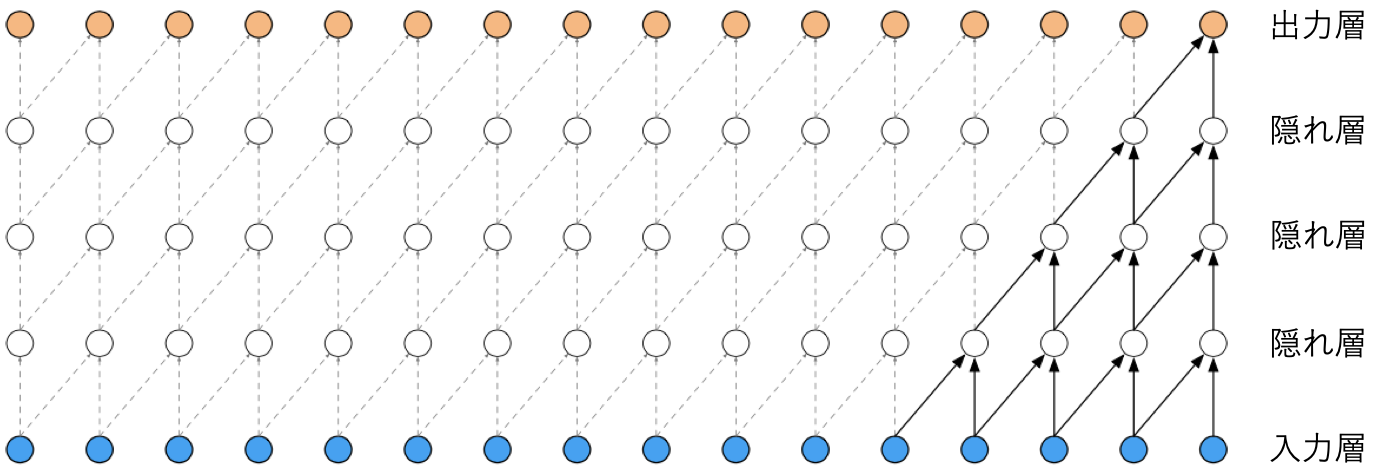
\includegraphics[width=\linewidth]{./figure/ccl.png}
	\caption{AlphaZeroのチェスのやつとconnect4と強化学習の式を合わせていい感じに}
	\label{fig:ccl}
\end{figure}
本論文で使用したalphazero baselineにおける入力は最新の盤面の状態を空白を0, 先番(赤)の石の位置を1, 後ろ
番(黄)の位置を-1として抽象化した6$\times$7の行列となる。
また、後述するconnect4のルール上の制約により次にプレイヤーが打つ箇所(行動)は列の数と同数の7つに限定される。

\subsection{AlphaZero}
AlphaZeroは2016年に登場し、元世界チャンピオンであるイ・セドルに対して四勝一敗の成績を収めたAlphaGoの汎用版である。
AlphaZeroは先述の$V(s),Q(s, a)$を推定する際にニューラルネットワークとモンテカルロ木探索システムを使用する。
\paragraph{ニューラルネットワーク}
AlphaZero内のニューラルネットワークに対する入力は最新$N$ステップの盤面($\left\{ s_{-N+1}, ..., s_0 \right\}$,$s_{-i}$は$i$ステップ前の盤面,$s_{0}$は現在の盤面)であり、出力は方策$P(\left\{ s_{-N+1}, ..., s_0 \right\})$と
局面評価(後で確認)$V(s_0)$の二種類である。\
ネットワークの構成は 層の残差結合ネットワークである。方策は「現在の状況$s_0$から次にどこを選択すべきか」を表現しており、次に選択すべき座標を確率分布の形式で表現する。
alphazero baselineにおける選択肢は列の数と等しい7であるため、1$\times$7の行列となる。方策内の値が大きさがAIによるその着手の評価と解釈され、成分が大きい座標を次に選択することが推奨される。例えば方策が
$\left\{0, 0.1, 0.2, 0, 0, 0.7, 0.8\right\}$であるとき、方策中の最も大きい成分は7番目の0.8であるため、プレイヤーは次に7列目を選択する事が推奨される。
また、局面評価$V(s_0)$は「現在の状況$s_0$は勝利に近いのか」を表現しており、値が上限に近ければ近い程、現在の状況$s_0$が次の着手を選択するプレイヤーにとっての勝利に近いことを表している。

訓練とかどうするん?
\begin{figure}[t]
	\centering
	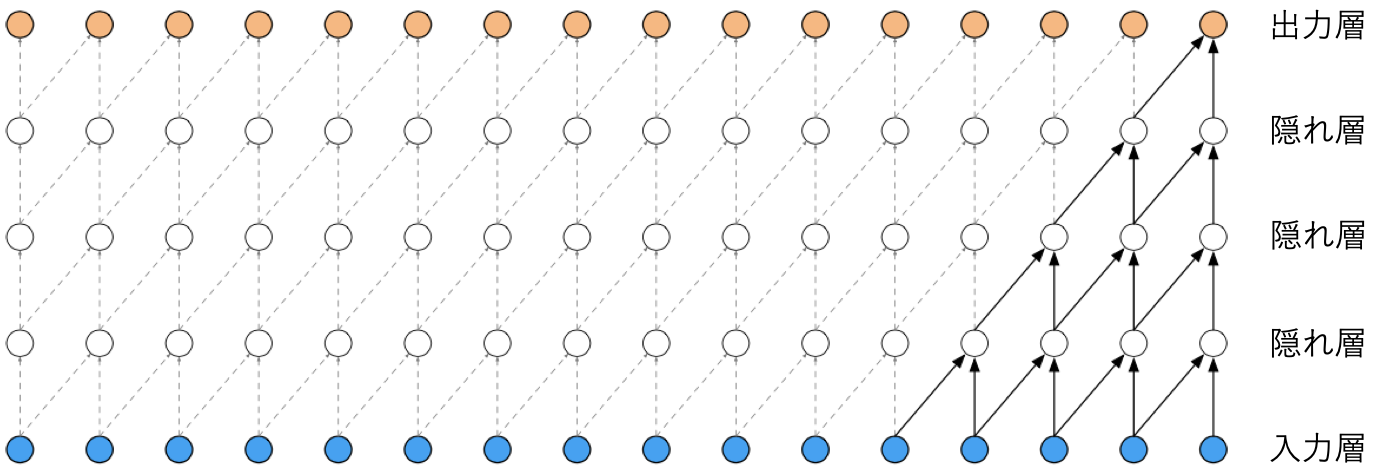
\includegraphics[width=\linewidth]{./figure/ccl.png}
	\caption{方策と局面評価、あと残差結合の図も}
	\label{fig:ccl}
\end{figure}
\paragraph{モンテカルロ木探索}
モンテカルロ木探索ではニューラルネットワークから得た方策$P(s)(以下s=\left\{ s_{-N+1}, ..., s_0 \right\}とおく)$と局面評価$V(s)$をシミュレーション
によって改善する。
モンテカルロ木探索ではシミュレーションによって各状態$s$をノード、各行動$a$を枝とした決定木を構築する。
最終的に各ノード$s$から派生する各行動$a$の分布$\left\{a_0, a_1, ..., a_n\right\}$が改善された方策となる。
一方、局面評価もまたモンテカルロ木探索により決定木が拡張されるなかで更新される。以下に決定木と局面評$V(s)$の更新アルゴリズムを示す。
表アルゴリズム\ref{table:result-1}
step1ではまず、探索の開始地点となるノード$s$を決定する。次にStep2:再帰部分では以下の処理を再起的に呼び出す。
\begin{enumerate}
	\item ノードを探索したことがない場合
	ニューラルネットワークから出力された方策$P(s)$と局面評価$V(s)$を返却する
	\item ノードを探索したことがある場合
	以下のpuctスコアに従い、子ノード$s_c$を選び、$s_c$に対して探索を行いその結果である$P(s_e), V(s_e)(s_eは再帰処理の結果たどり着く
	決定木の端のノード)$を受け取る。
\end{enumerate}

$P(s_e), V(s_e)$を用いて
パラメータをこんなふうに更新する。

このようなプロセスによって構築された決定木を用いてモデルは対戦を行う。
\subsection{AlphaZeroの問題点}
StockFish\cite{oord2016wavenet}やなんか\cite{oord2016wavenet}などの従来のボードゲームAIはそのゲーム固有の知識(ドメイン知識)に基づくものが多く、「ある条件を満たすときにある選択をする」と言ったようにその挙動をルールとして表すことが可能である。
一方でこのニューラルネットワーク+木探索の手法では
人間がネットワークから得られる情報は方策と局面評価のみである。その他のパラメータも観察可能ではあるが、その方策や局面評価の根拠を得ることができない、つまりAlphsZeroの問題点として説明性の欠如が挙げられるのである。
説明性の欠如はAIの判断に対する責任の不在を意味し、優れた性能を持つシステムのより、ハイレベル、ハイリスクなタスクへの実用化に対する障害となる。



\section{XAI}

\subsection{概要}
XAIとはexplainable AI(説明可能AI)の略語であり、AIを人間に対して説明可能なものにする、もしくは説明可能なAIを構築する領域である。
本論文はAIの判断根拠として先読みを示す意味でXAIの分野に属する研究であると言える。
ここでの「説明可能性」の語は「人間に理解できる形での説明を与える能力」\cite{oord2016wavenet}と定義され、
「いつ、どのような、どのように」説明を与えるかによってさらに細かく分類される。
「いつ」、つまりどの時点で説明を与えるか、に関しては既存のネットワークに対して新たに説明を加える「事後的」説明と初めから動作の根拠を示せるようにネットワークやシステムを構築する「事前的」説明
に分類できる\cite{oord2016wavenet}。
「どのような」、つまり説明の内容については
が存在する。
また、「どのように」つまり説明を表現する形態としてはsaliency map, Grad-CAM\cite{oord2016wavenet}といった視覚的な可視化や、あとで
\cite{oord2016wavenet}といった文章生成等が存在する。
本論文において構築するシステムは「事後的」「局所的」「視覚的」説明を提供する。

Wavenet\cite{oord2016wavenet}は
音声波形を時系列データとして自己回帰モデルで学習することによって,人間の声のような自然な音声を生成することができる.
時点$t$における観測値を$x_t$,$\bm{x} = \left\{ x_1, ..., x_T \right\}$を観測値の全体集合とする.このとき,波形の同時確率は条件付き確率の積として
以下のよう表現される.
\begin{equation}
	p(\bm{x}) = \prod_{t=1}^T p(x_t | x_1, ..., x_{t-1})
\end{equation}

つまり,$x_t$は前時点の全てにおけるサンプルに条件づけられる.
また、本論文は
XAI分野の中でも特に強化学習方面に対して説明を加える領域をXRL(explainable Reinforcement learning)と呼ぶ。XRLの試みは様々な強化学習システムを対象とし、
\subsection{ボードゲームにおけるXAI}
グーグルのやつはチェスにおける人間の知識がAlphaZeroにどれだけ反映されているかを訓練段階やネットワークの深さなどの多様な指標で調査している。\cite{oord2016wavenet}
ディコードチェス\cite{oord2016wavenet}はAIの着手に対して、そのゲーム固有の知識(以下ドメイン知識と記載する)を用いて解説を生成する 
しかし、このようなドメイン知識が必ずしもAIの挙動と相関が無いことも指摘されている。\cite{oord2016wavenet}
AIによる画像分類の可視化手法であるサリエンシーマップ\cite{oord2016wavenet}やGrad\_CAM\cite{oord2016wavenet}を強化学習に用いる例も存在する。しかしそれらのニューラルネットワークの活性を根拠とした指標は木探索部分との繋がりが弱く、最終的に決定木を用いて意思決定を行うシステムの動作根拠を直接的に説明できない。
また、これらの画像分類用の手法は
\begin{itemize}
	\item 本来ゲームに存在する時系列の要素を説明に含められない
	\item 時系列を無視してゲーム画面や盤面の一部を変更する必要がある
\end{itemize}
という問題点が存在する。

\subsection{contrastive explanation}
上述の問題点を解決するために、本論文ではAlphaZeroが構築する決定木を用いたcontrastive explanation(対象説明、比較説明)を提供する。
contrastive explanationは事象を説明する際の方法論の一つであり、
ある事象$a$が起こった際にその理由を直接説明する代わりに「他の事象$\bar{a}$が起こらなかった理由」を説明することで間接的にある事象$a$の原因を説明するアイデアである。
 では言語の何か \cite{oord2016wavenet}ではニューラルネットワークの判断を決定木に近似した上でニューラルネットワークの判断$a$から派生する予想と別の判断$b$から派生する予想を同時に提示する。
ロボット\cite{oord2016wavenet}の、ではある時点$t$で異なる行動を選んだ場合の結果の違いを文章で説明する
アミア\cite{oord2016wavenet}では異なるシステム間の特徴をユーザーに示す目的でcontrastive explanationが用いられている。

\subsection{ボードゲーム学習支援}
本論文が提案する手法は高いパフォーマンスを発揮するAIの動作を人間に理解させることを目標としており、学習支援の面を持つ。
既存のAIを用いたボードゲーム学習支援システムとしてはドメインみたいなやつをいくつか
が存在し、決定木の先読みを用いて文章生成や解説生成を行う。
しかし「ボードゲームに対するXAI」の段での内容と同様にその多くがゲームのドメイン知識に依存しており、指導の内容も人間の知識に依存したものになってしまうという欠点がある。




\chapter{提案手法の概要}
関連研究の章ではニューラルネットワークや決定木が内包する説明性の欠如という問題点と説明を加える既存手法の持つ課題について述べた.
そこで,システムの決定木から結果に類似性のある複数の分岐を抽出することによる
\begin{itemize}
	\item 本来ゲームに存在する時系列の要素を含む
	\item 評価基準が勝敗に直結する
    \item 人間のドメイン知識に依存しない
\end{itemize}
説明手法を提案する.
図\ref{fig:mabs}に示すように本手法はある状態$s$と行動$a$の組に対してAIによる予想図の集合$\alpha$とそこに至るまでの軌跡の集合を取り出す.そしてその傾向を見出すことによるAIの判断
の意図の可視化を目標とする.
以降は予想図の集合$\alpha$と走査が$\alpha$に至るまでに通過したノードの履歴(軌跡)$\zeta$を合わせて進行図と記載する
\begin{figure}[htbp]
    \centering
    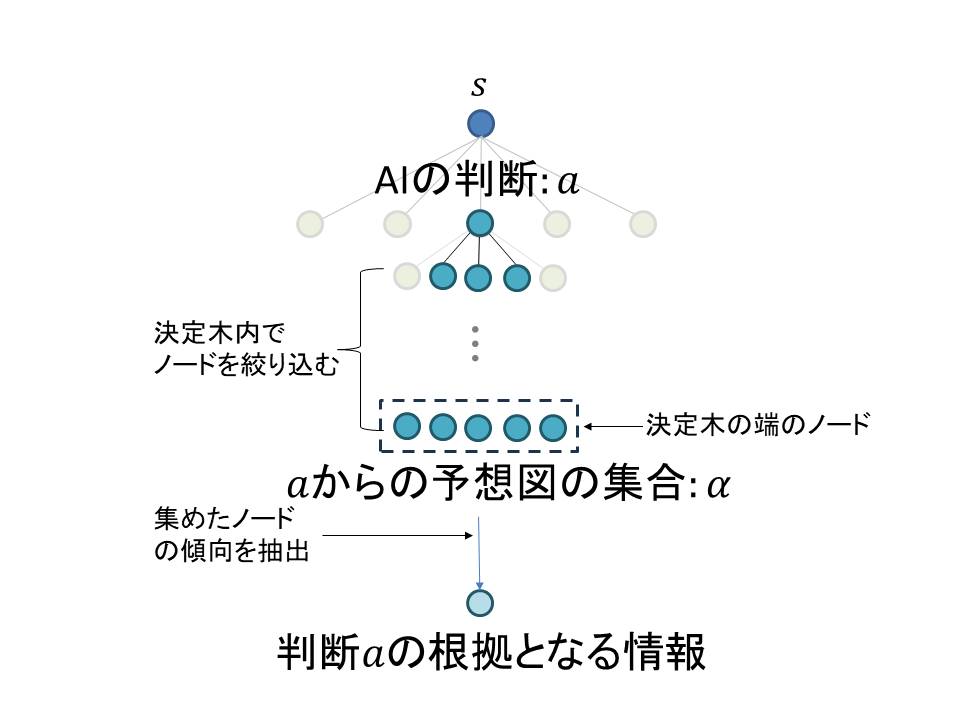
\includegraphics[width=\linewidth]{./figure/mabs.png}
    \caption{提案手法の概要}
    \label{fig:mabs}
\end{figure}
本章では提案手法のアルゴリズムと,第2章で述べた重要度$I(s)$の新たな定義を記載する.
それから,
実験のタスクとして選択したconnect4,使用したモデルであるalphazero\_baseline,そして提案手法のconnect4への応用例について記載する.


\section{提案手法のアルゴリズム}
本手法はAlphaZeroシステムのニューラルネットワークと木探索部分のうち,主に木探索の部分を対象に適用される.
本手法では決定木の判断を説明する際に最も有用な部分を決定木から抽出することを主な目的としており,アルゴリズムはボードゲームAIに留まらず決定木構造を持つ多くのシステムに応用可能である.
アルゴリズムの流れは以下の通りである.
図\ref{fig:step1-2},図\ref{fig:step3-4}はステップごとのアルゴリズムの概要である.
\begin{enumerate}
    \item 説明を付与する状態(図\ref{fig:step1-2}の青いノード)と行動の組$(s_{start}, a)$を選択する.
    このとき注目している状態$s_{now}, a_{now}$はそれぞれ
    \begin{equation}
        {s_{now}=s_{start}}
    \end{equation}
    \begin{equation}
        {a_{now}=a}
    \end{equation}
    とする.
    \item 以下の流れを$l$ステップ分繰り返す.\\
    決定木中の注目しているノード$s_{now}$からの探索回数が上位$k$個分の行動$\{a_1, a_2, ..., a_{k}\}(a_iはk番目に探索回数の大きい行動とする)$を取り出す.
    $s_{now}$から行動$\{a_1, a_2, ..., a_{k}\}$を取ることでたどり着く各ノード\\
    $\{s_{next_1}, s_{next_2}, ..., s_{next_{k}}\}(s_{next_i}=T(s_{now}, a_i), Tは遷移関数)$に対して同様の操作を繰り返す.
    図\ref{fig:step1-2}に示すように,結果的に$k^l$個のノードが取り出される.
    
    \item 集めた$k$の$l$乗個のノード$\{{s}'_{1}, {s'}_{2}, ..., {s'}_{k^l}\}$のそれぞれ${s'}_{i}(i=1, 2, ..., k^l)$に対して以下の操作を再帰的に繰り返す.
    ${s'}_{i}$における方策$P({s'}_{i})$中の最も有望な(探索回数の大きい)行動$a_{promising}$と${s'}_{next_i}=T({s'}_i, a_{promising})$を記録する.
    そのようにして記録した$\{{s'}_{next_1}, {s'}_{next_2}, ..., {s'}_{next_{k^l}}\}$中のそれぞれの${s'}_{next_j}(j=1, 2, ..., k^l)$にも同様の操作を盤面ノードが決定木の端に辿り着くまで行う.
    結果的に$k^l$個の葉ノード(図\ref{fig:step3-4}下部の紫色のノード)が集められる.
    \item 3.によってたどり着いた$k^l$個のノードによる集合$S=\{s_{edge_1}, s_{edge_2}, ..., s_{edge_{k^l}}\}$を任意の共通項$c$によっていくつかの副集合$\{S_1, S_2, ..., S_q\}$に分ける.
    \item 共通項で括られた各集合$\{S_1, S_2, ..., S_q\}$のうち,最も要素数が多いもの$S_{max}$中の各要素$\{s_{e_1}, s_{e_2}, ...,  s_{e_u}\}$と各要素に対応する軌跡$\{\rm{{\zeta}_{s_{e_1}}}, \rm{{\zeta}_{s_{e_2}}}, ...,  \rm{{\zeta}_{s_{e_u}}}\}$を抽出する.
    図\ref{fig:step3-4}では青い点線で囲われたグループが抽出される.
    ここでの軌跡$\rm{{\zeta}_{s_{e_i}}}$とは,図\ref{fig:traj-example}に示すように決定木を走査する際に$s_{start}$から$s_{e_i}$にたどり着く際に,どのような状態$s$や行動$a$を経由したかを表している.
    図\ref{fig:traj-example}における$\rm{{\zeta}_{s_{e_i}}}$は$\{s_{start}, a_1, s_1, a_2, s_2, a_3, s_3, a_4, s_{e_i}\}$となる.

\end{enumerate}


\begin{figure}[htbp]
    \centering
    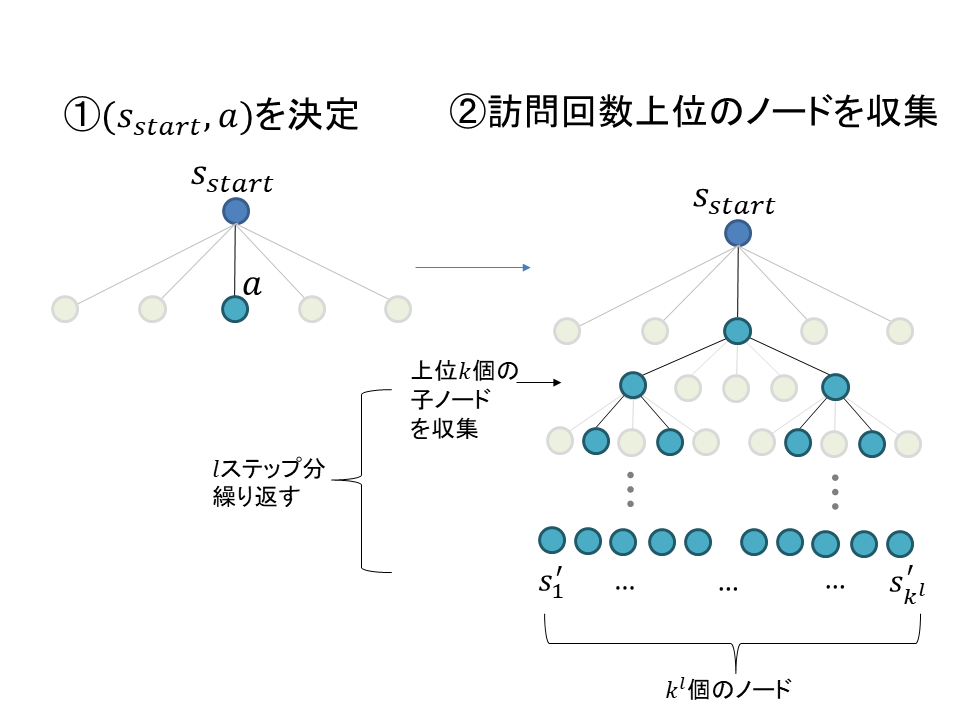
\includegraphics[width=\linewidth]{./figure/1-2.png}
    \caption{提案アルゴリズムの概要(step1$\sim$ 2)}
    \label{fig:step1-2}
\end{figure}
\begin{figure}[htbp]
    \centering
    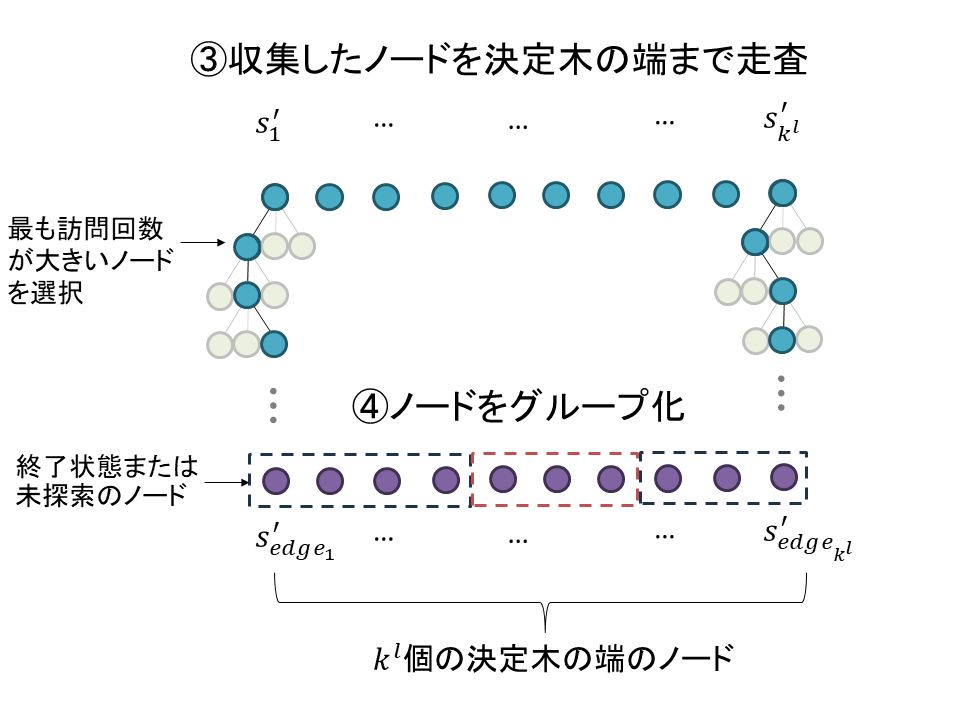
\includegraphics[width=\linewidth]{./figure/3-4.png}
    \caption{提案アルゴリズムの概要(step3$\sim $4)}
    \label{fig:step3-4}
\end{figure}
\begin{figure}[htbp]
    \centering
    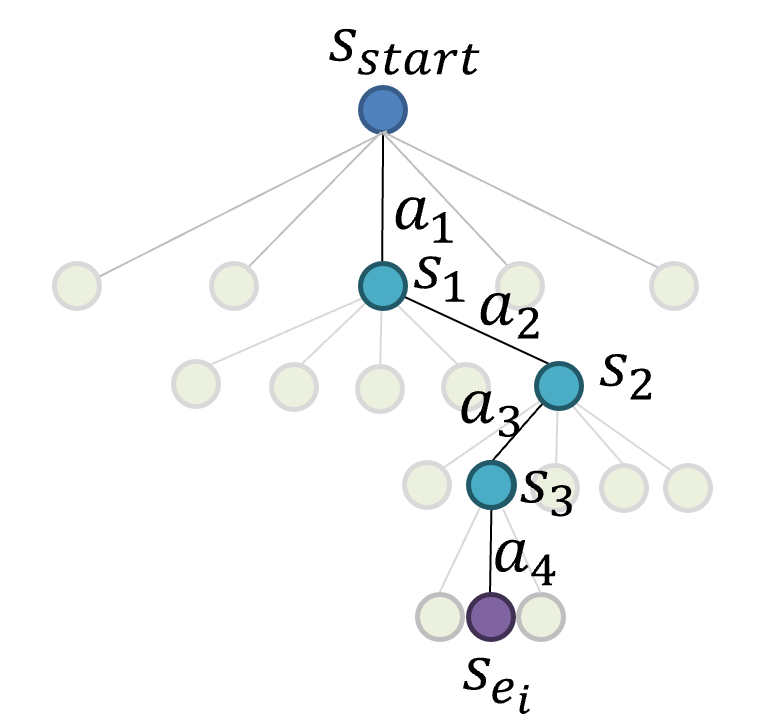
\includegraphics[width=200pt]{./figure/traj-example.png}
    \caption{軌跡の例}
    \label{fig:traj-example}
\end{figure}
このアルゴリズムを要約すると,図\ref{fig:merit}のようにある局面$s$と行動$a$の組み合わせから辿り着きやすい結末$O(s, a)$を抽出し,同時に$O(s, a)$に至るまでの複数の軌跡を抽出すると表現できる.
調査を行う者が複数の軌跡を観察できることで,
共通する傾向や法則性を見出せるというメリットが存在する.これは第2章で述べたような最も可能性が高い1つの軌跡を示す,といったような情報が単一である従来の手法には不可能である.
提案手法の疑似コードは付録\ref{chap:alg}に記載している.

\begin{figure}[htbp]
    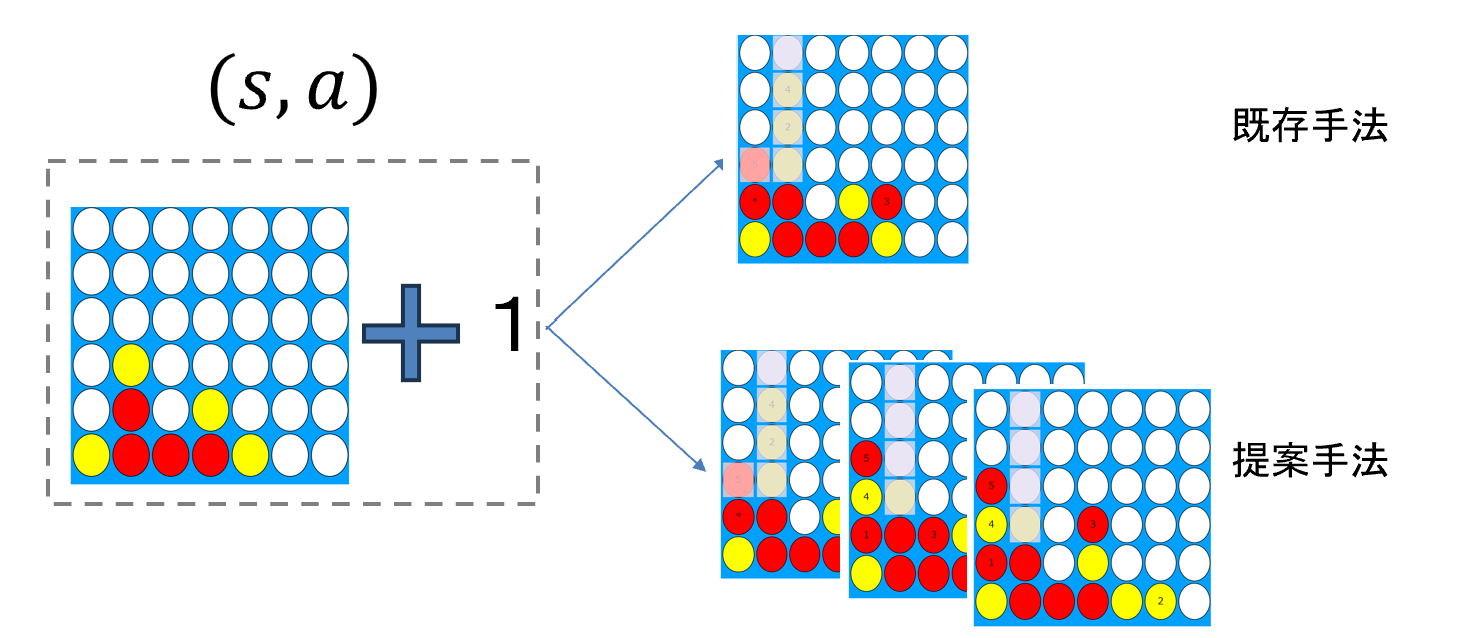
\includegraphics[width=400pt]{./figure/merit.png}
	\caption{提案手法と既存手法}
	\label{fig:merit}
\end{figure}




付録\ref{chap:data}で示すようにconnect4タスクにおいて収集される軌跡の集合においては末端部分のいくつかの選択が共通している傾向が確認された.
そのため状態と行動の組$(s, a)$から$O(s, a)$という結果を予測する過程で$O(s, a)$から末尾の数手を取り除いた版面$d$にたどり着く傾向の発見などの知識獲得が期待される.
\section{importance}
前章で述べたように,エピソード中の各状態$s$の重要度$I(s)$の定義を以下のように定めた.
\begin{equation}
    \label{new-imp}
	{I(s)=V[Q'] (Q'=[\rm{Max}Q(s, a), \rm{SecondMax}Q(s, a), ..., \rm{ThirdQuantile}Q(s, a)])}
\end{equation}
つまり,現在の状態$s$に対する行動の集合$A(={a_1, a_2, ..., a_N})$とした際の行動価値関数の集合${Q(s, a_1), Q(s, a_2), ..., Q(s, a_N)}$のうち値の大きさが上位75
\%の成分で構成される集合の分散として重要度$I(s)$を定義する.
上位75\%の成分のみを使用し,平均の代わりに分散を使用したこの定義により,先述した盤面の対称性や悪い選択肢の影響の軽減が期待できる.

\section{connect4}
connect4はボードゲームの一種である.ルールは五目並べに極めて近く,図\ref{fig:connect4}の右側の画像のように,2人のプレイヤーが交互に互いの駒を盤上に置き,最終的に縦,横,もしくは斜めに連続して4つの石を並べたプレイヤーの勝利となる.ただし,五目並べや連珠との相違点として「重力」の存在が挙げられる.
この「重力」とは各プレイヤーが石をボード上の最も下の行または既に置かれた石の上にしか置けないという規則を表している.そのため,各プレイヤーの選択肢はボードの列の数と等しい.
図\ref{fig:connect4}の左側は左から5番目の列を指定した際に,石がボード上の最下の列に置かれる様子を示している.
connect4の一般的なボードの広さは$6\times7$であり$6\times7$のコネクト4については1988年にAllis\cite{allis}により知識ベースの手法による先番勝利が証明された.
Tromp\cite{data}によるconnect4の$\alpha-\beta$木探索によって導かれた各盤面の最善手とそのデータも一般に公開されている.
また,connect4は盤上に全ての情報が開示されており,結果もどちらか一方の勝利または引き分けのみであるため2人ゼロ和完全情報ゲーム\cite{gairon}に分類される.
本論文の実験において提案手法をconnect4に適用する際には最終盤面において4つ以上並んでいる石の座標を特徴として用いた.
\begin{figure}[htbp]
	\centering
    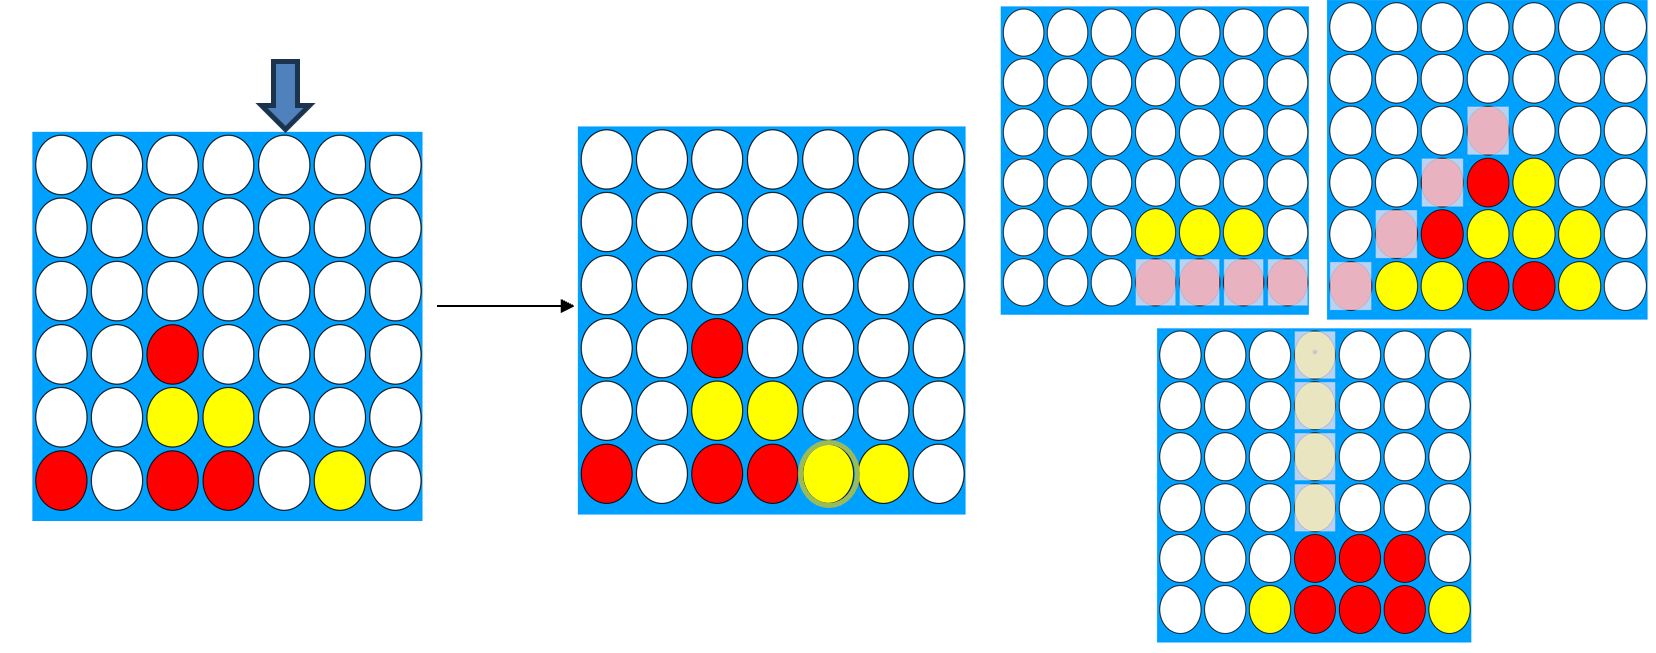
\includegraphics[width=\linewidth]{./figure/connect4.png}
	\caption{connect4}
	\label{fig:connect4}
\end{figure}
\section{alphazero\_baseline}
alphazero\_baselineはalphaZeroをconnect4用に簡易的に模したネットワークであり,図\ref{fig:baseline}に示すように入力は最新の盤面$s_0$,出力は$1\times7$(7はボードの列の数)の方策$P(s)(以下s=s_0とする)$とスカラー値の局面評価$V(s)$(値域は-1から1)である.
方策は確率分布であり,要素の値が大きいインデックスを選択することで勝利に近づくと予想される.
局面評価は第2章の強化学習の段で記載した状態価値関数と同一の変数である.
局面は状態$s$に対する評価を表しており,1が入力の手番のプレイヤーにとっての勝利,-1が敗北の予想を表している.

\begin{figure}[htbp]
    \centering
    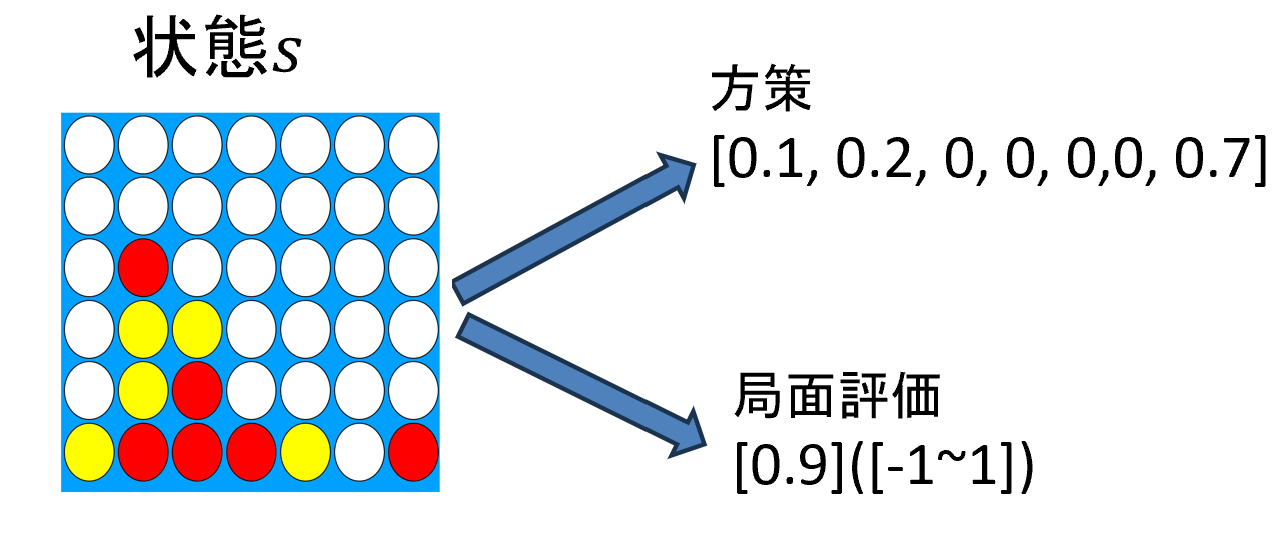
\includegraphics[trim={0cm 0cm 0cm 0cm},clip]{./figure/baseline.png}

    \caption{alphazero\_baselineの入出力}
    \label{fig:baseline}
\end{figure}
\section{提案手法のconnect4への適用}
提案手法をconnect4に適用した際の概要を図\ref{fig:application}に示す.進行図は1組の盤面$s$と行動$a$に対して決定木中の有力なノードを走査することで生成される.
提案手法をconnect4に適用する際,各ノードはalphazero\_baselineへの入力であるconnect4の各盤面となる.

また,ゲームのルールより,収集される最終状態では図\ref{fig:application}の下部のように4つ以上並んだ石が存在する.
第4章で詳しく述べるように,実験では4つ以上並んだ石の位置で最終状態をグループ化した.図\ref{fig:application}においては石が左下から右斜め上方向に4つ並んでいる盤面
が最も多いため,赤線で囲われた盤面とそこにいたるまでの軌跡が保存される.
\begin{figure}[htbp]
	\centering
	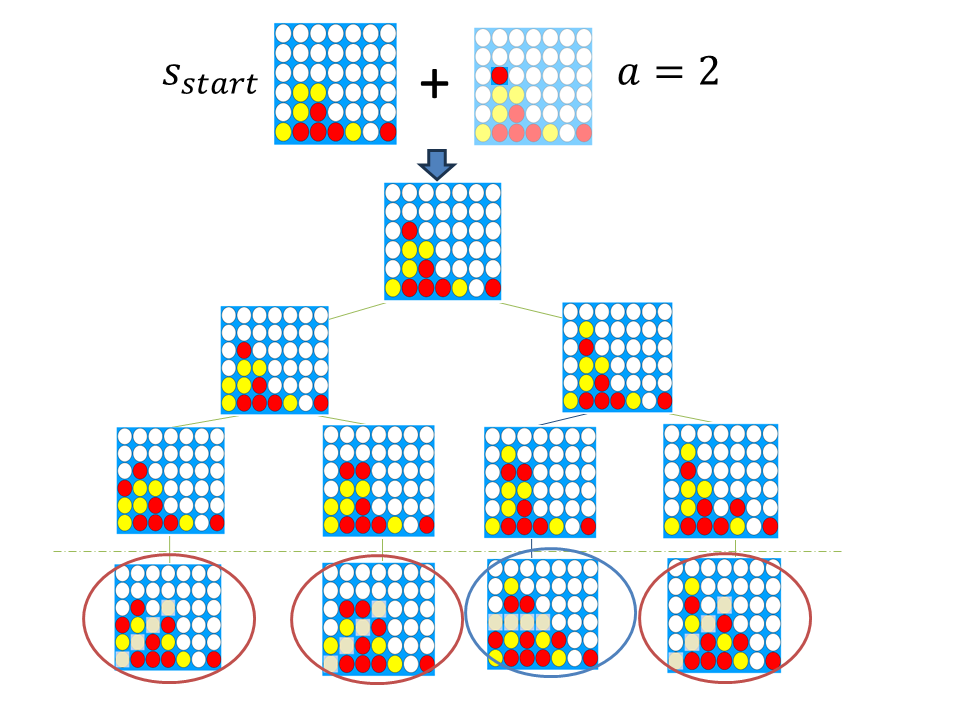
\includegraphics[width=\linewidth]{./figure/application.png}
	\caption{提案手法のconnect4への適用}
	\label{fig:application}
\end{figure}

提案手法により生成される進行図を図\ref{fig:double}に示す.
先述のように進行図は予測図と軌跡で構成されている.connect4では盤面$s$と行動$a$を選んだ際の次の状態$s_{next}$は$(s, a)$に対して一意に決定される.
そのため,軌跡$\rm{{\zeta}_{s_{e_i}}}$は$s_{start}$から$s_{e_i}$に至るまでに取った行動$a$の集合とした.各行動は選択した列のインデックスで$1\sim7$の数字として
表現される.
\begin{figure}[htbp]
	\centering
	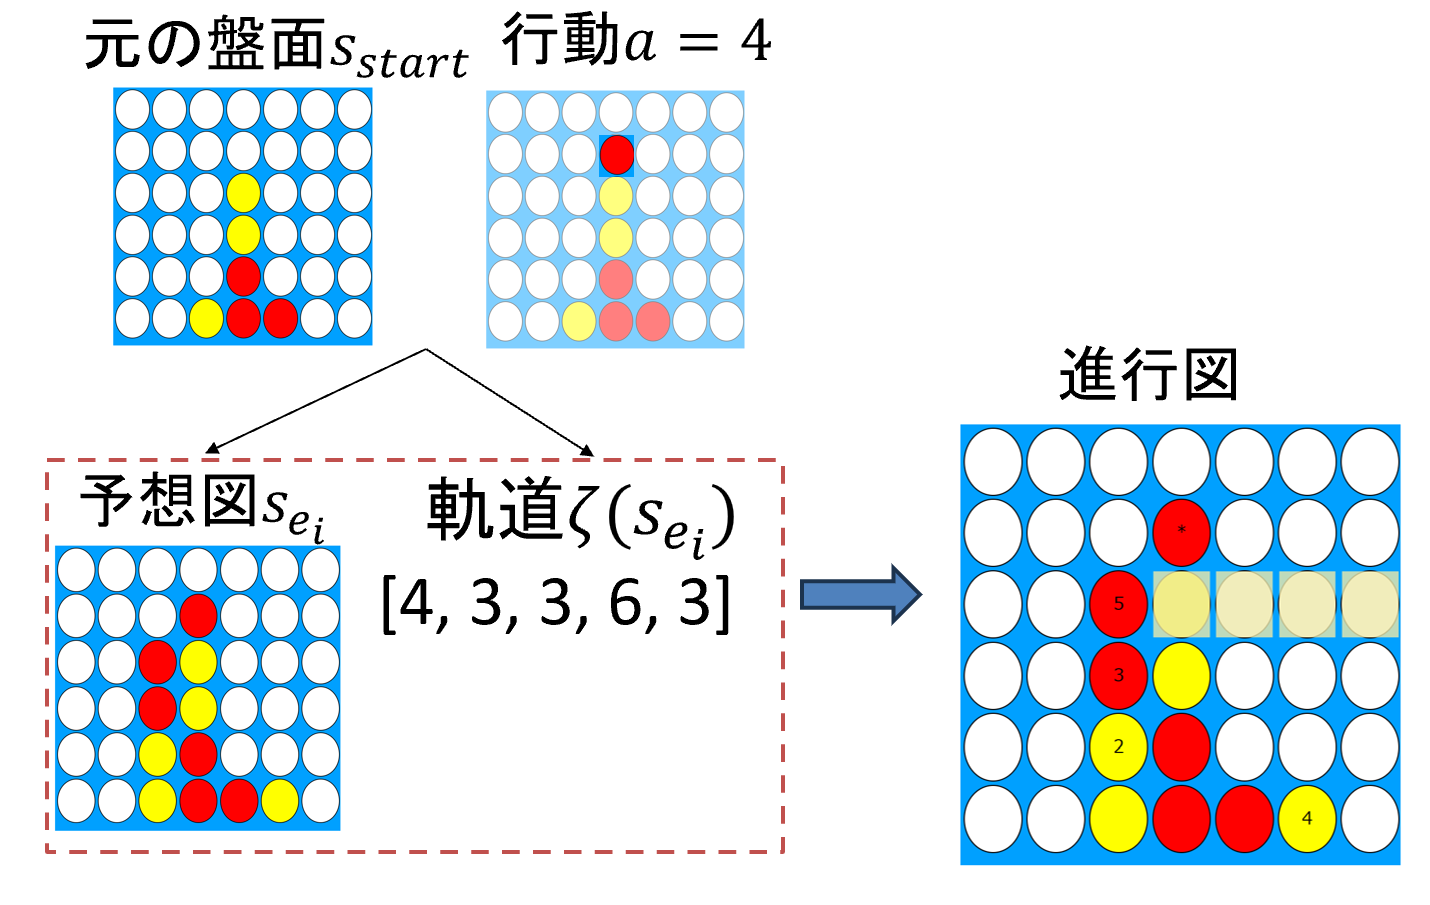
\includegraphics[width=\linewidth]{./figure/double.png}
	\caption{connect4における進行図}
	\label{fig:double}
\end{figure}
\pagebreak
\chapter{評価実験}
提案手法の有効性を示すため2種類の実験を行った。いずれもタスクの対象としてconnect4を扱っている。\\
一つ目の実験(以下データ実験と表記)はコンピュータ同士の対戦データを用いて提案手法による想定図の妥当性の実証を試みた。\\
二つ目の実験(以下システム実験と表記)は自作のconnect4学習支援システムを用いて提案手法のユーザーインタフェースを含んだ優位性の実証を試みた。
この章ではまず実験の際に用いたタスクであるconnect4と使用したモデルであるalphazero\_baselineについて述べる。そののちにデータ実験、システム実験の詳細と結果を記載する。
\section{connect4}
connect4\cite{connect4}はボードゲームの一種である。ルールは五目並べに極めて近く、二人のプレイヤーが交互に互いの駒を盤上に置き、最終的に縦・横・もしくは斜めに連続して4つの石を並べたプレイヤーの勝利となる。ただし、五目並べや連珠との相違点として「重力」の存在が挙げられる。
この「重力」とは各プレイヤーが石をボード上の最も下の行または既に置かれた石の上にしか置けないという規則を表している。そのため、各プレイヤーの選択肢はボードの列の数と等しい。
connect4の一般的なボードの広さは$6\times7$であり$6\times7$のコネクト4については1988年にAllis\cite{allis}により知識ベースの手法による先番勝利が証明された。
Tromp\cite{data}によるconnect4の$\alpha-\beta$木探索によって導かれた各盤面の最善手とそのデータも一般に公開されている。
また、connect4は盤上に全ての情報が開示されており、結果もどちらか一方の勝利または引き分けのみであるため2人ゼロ和完全情報ゲームに分類される。
本論文の実験において提案手法をconnect4に適用する際には最終盤面において4つ以上並んでいる石の座標を特徴として用いた。
\begin{figure}[t]
	\centering
    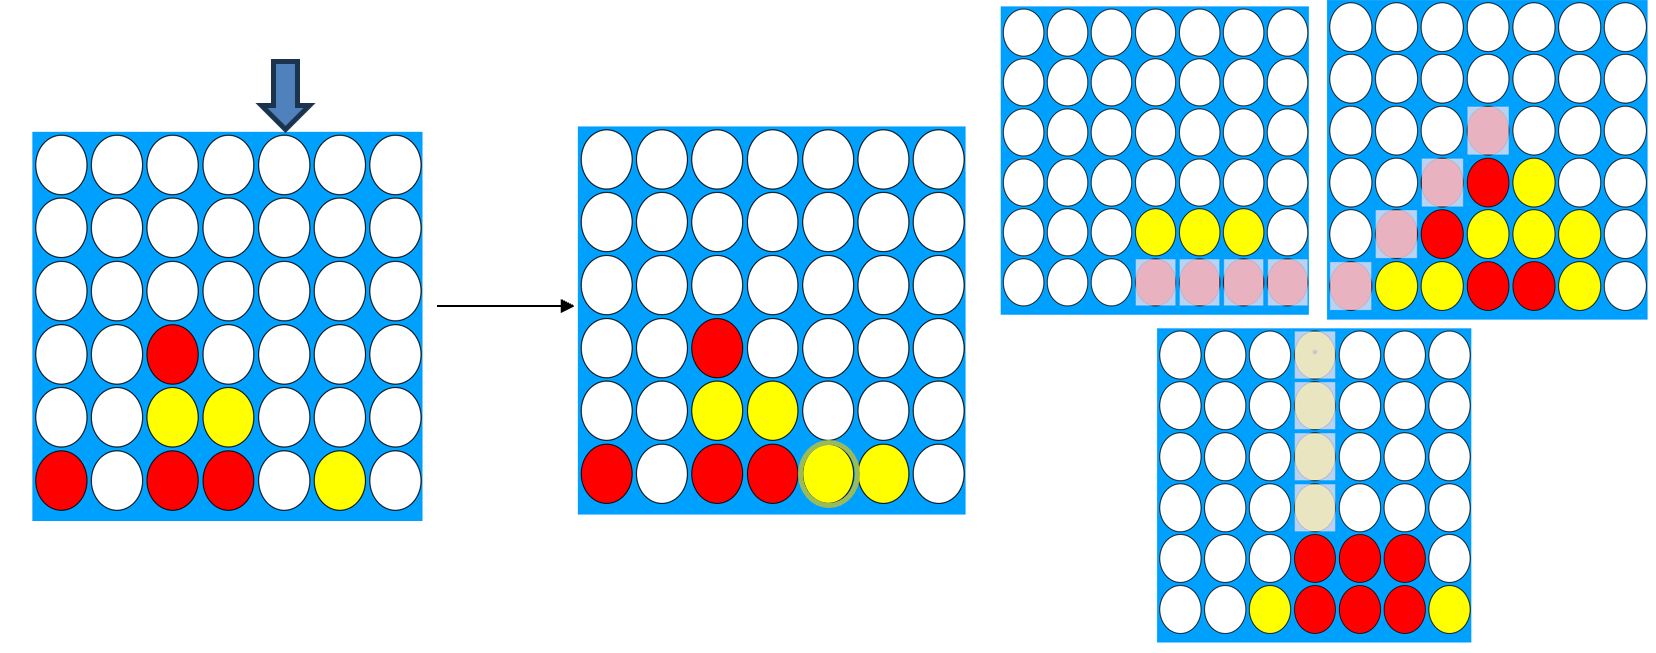
\includegraphics[width=\linewidth]{./figure/connect4.png}
	\caption{connect4}
	\label{fig:connect4}
\end{figure}
\section{alphazero\_baseline}
alphazero\_baseline\cite{baseline}はalphaZeroをconnect4用に簡易的に模したネットワークであり、入力は最新の盤面$s_0$、出力は$1\times7$(7はボードの列の数)の方策$P(s)(以下s=s_0とする)$とスカラー値の局面評価$V(s)$(値域は-1から1)である。
方策は確率分布であり、要素の値が大きいインデックスを選択することで勝利に近づくと予想される。
局面評価は第2章の強化学習の段で記載した状態価値関数と同一の変数であり、
入力に対する評価を表しており、1が入力の手番のプレイヤーにとっての勝利、-1が敗北の予想を表している。

\begin{figure}[t]
    \centering
    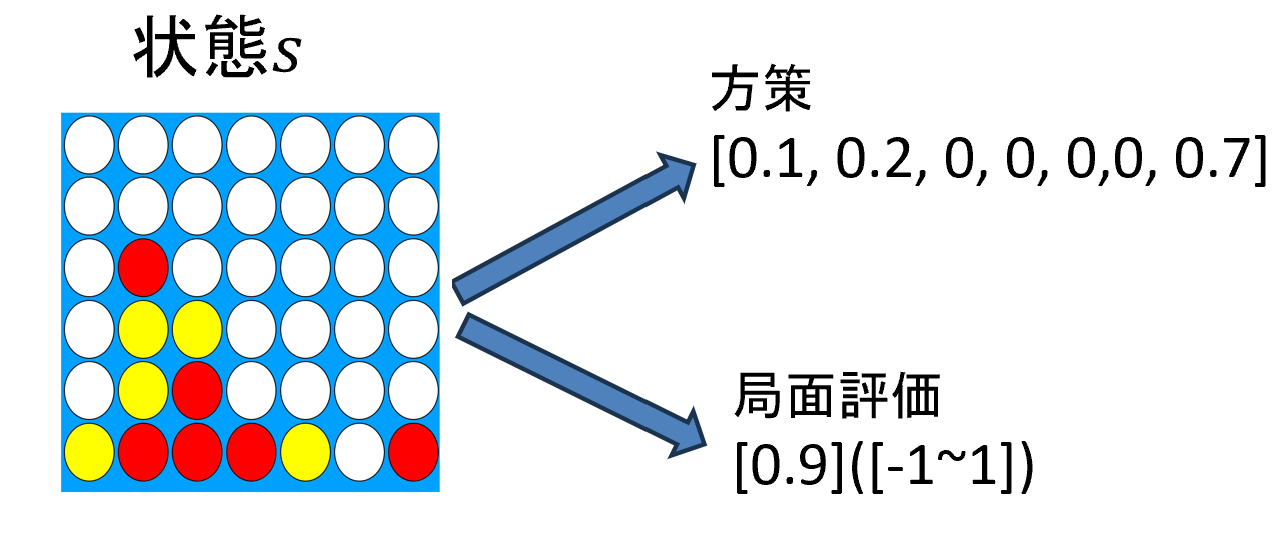
\includegraphics[trim={0cm 0cm 0cm 0cm},clip]{./figure/baseline.png}

    \caption{alphazero\_baselineの入出力}
    \label{fig:baseline}
\end{figure}


\section{データ実験}
\label{chap:evaluation}
提案手法と後に述べる比較手法によるゲーム結果(後で勝敗も含める)の予測精度を比較した。
\subsection{データセット}
alphazero\_baselinモデル同士の対戦データ2000局分(盤面数:61049)を使用した。いずれもいずれも弱いAIが先番のデータを使用している。これは弱いAIが後番の場合評価関数の変動が極めて小さくなることと、弱い側が先番を選択することが指導において一般的とされるためである。

\subsection{比較手法}
提案手法と比較手法はそれぞれ以下の方式で予測を行う。
比較手法の詳細なアルゴリズムは付録\ref{chap:alg}に記載した。
\newpage
\begin{itemize}
	\item 比較手法: 探索の開始地点から最も訪問回数が大きい選択肢を選び、決定木の端までたどり着いた際にそこで四つ繋がっている石の組み合わせ、位置を記録する。
	\item 提案手法: 集めた盤面における4つ繋がっている石を集計し、出現頻度が高い4つの個別の石の位置と出現頻度が高い二つの組み合わせを記録する。組み合わせを二つ記録する理由は下の図のように最終的に繋がっている組み合わせが二つある可能性を考慮するためである。
\end{itemize}
図\ref{fig:compare}は比較手法の概要を示している。
\begin{figure}[t]
	\centering
	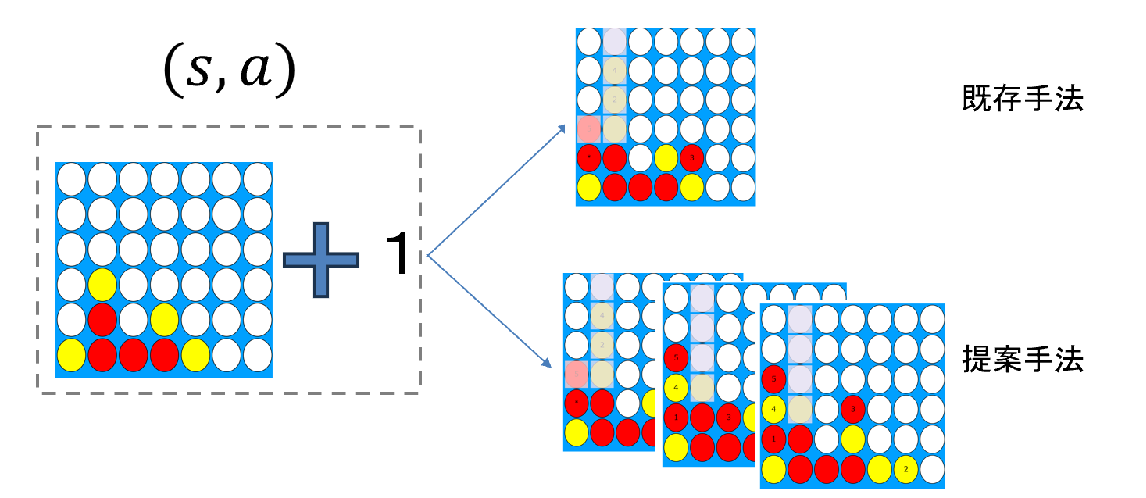
\includegraphics[width=\linewidth]{./figure/compare.pdf}
	\caption{提案手法と比較手法の比較}
	\label{fig:compare}
\end{figure}

\subsection{評価指標}
両手法による予測の精度を独自に定義した二つの定義group count($C_g$)、stone count($C_s$)によって計測した。stone count、 group countの詳細な定義は付録Aに記載する。
それぞれが、最終盤面において4つ以上連続して並ぶ石と組み合わせ(以下fatal stone、fatal groupと記載)の座標に対する予測精度を表している。
ここでは概略を述べる。
手法によって予測されたfatal stone、fatal groupの座標をそれぞれ$F_s, F_g$とする。

\paragraph{group count}~
\par 予測の石の組み合わせ単位での精度を示しており、
手法による予測$F_g$と実際のfatal groupの集合$R_g$に共通する要素がある場合1、無い場合は0となる。
また、$F_g$と$R_g$が両方とも空集合$\phi$である場合(実際の結果が引き分けでありかつそれを正しく予測できている場合)group countは1となる。
\paragraph{stone count}~
\par 予測の個別の石単位での精度を表しており、
手法による予測$F_s$と実際の集合$R_s$の共通する要素の数を4で割った値である。値の最大値は1であり、先述の値が1を超える場合もstone countは1として扱う。
group countと同様に$F_s$と$R_s$が両方とも空集合である場合stone countは1となる。
\subsection{実験結果}
盤面データのうち、手数(盤面上の赤または黄色)が13$\sim$24のものに対して実験を行った。
表\ref{table:result-online}に実験結果を示す。いずれの場合もgroup countにおいて提案手法は比較手法より高い値を示した。
表中に記載した「補間」の詳細は付録\ref{chap:alg}に記載する。
\begin{table}[H]
	\caption{実験結果:データ実験}
	\centering
	\scalebox{0.98}[0.98]{
		\begin{tabular}{c|c|c|c|c}
			\multicolumn{1}{c}{} & \multicolumn{2}{|c|}{group count} 
			& \multicolumn{2}{c|}{stone count}\\ \hline \hline
			手数(盤面数, 補間の有無)    & 提案手法 & 比較手法 & 提案手法 & 比較手法 \\ \hline
			19-24(9862, 無)    & \bf{0.60} & 0.43 & 0.55 & \bf{0.62} \\
			19-24(9862, 有)    & \bf{0.63} & 0.44 & 0.61 & \bf{0.63}  \\
			13-24(21022, 無)   & \bf{0.52} & 0.37 & 0.55 & \bf{0.56}  \\
			13-24(21022, 有)   & \bf{0.55} & 0.37 & 0.55 & \bf{0.56}  \\
		\end{tabular}
	}
	\label{table:result-online}
\end{table}
\subsection{考察(データ実験)}
提案手法はgroup countにおいて比較手法より高い結果を示した。
この結果は提案手法がfatal groupを予測する能力に長けている事を意味する。
比較手法によって予測されるfatal groupの集合は
最も訪問回数が大きい分岐が辿り着く1つの最終状態のものである。
一方で提案手法により予測されるfatal groupの集合は、複数の分岐がそれぞれに辿り着く最終状態のfatal groupの多数派投票によって決定され、第1位と第2位のものが採用される。\\
使用した対戦データは対戦者間の強さに差があり、予測は強い側の決定木を用いている。
決定木内での最も訪問回数の大きい分岐(以下主分岐と記載)はAIが予測する双方が最善を尽くした場合の進行と解釈される。
実際に弱いAIと対戦を行う際には、弱いAIは強いAIが最善とみなす行動(最も訪問回数が大きい行動)を必ずしも選択しない。
そのため、実際の進行は、比較手法に用いられる主分岐とは異なる可能性が高い。
提案手法では、主分岐を含む複数の分岐を用いているため、より精度の高い予測が可能になったと考えられる。\\
また、提案手法は2組のfatal groupを保存することから比較手法よりも予測するfatal groupの数が多くなる傾向にあるため、必然的にgroup countの値も大きくなったとも考えられる。


\section{システム実験}
提案手法の人間に対する有効性を示すため以下のような自作したconnect4の学習支援システムを用いて実験を行った。
実験対象者は計22人の10代-20代学生(男性17名:女性5名)となった。
\begin{figure}[t]
	\centering
	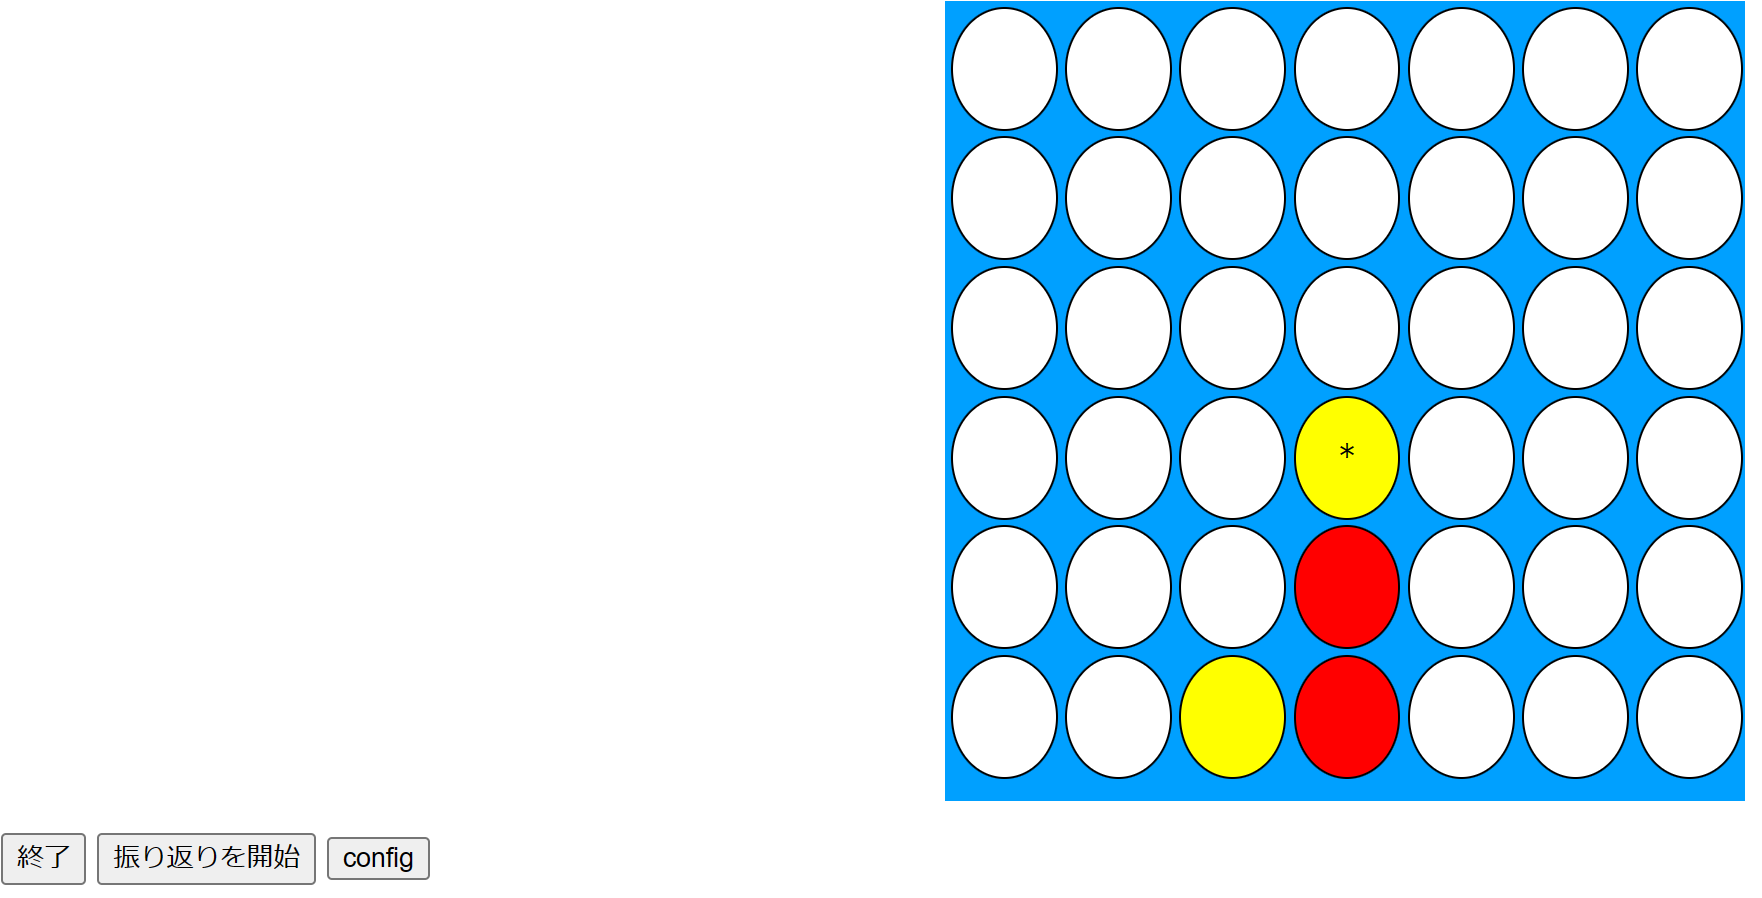
\includegraphics[width=\linewidth]{./figure/basicSystem.png}
	\caption{開始画面}
	\label{fig:basic}
\end{figure}
\subsection{実験手順}
実験は被験者一人あたりにつき三回行われ、前半二回を第一段階(提案手法による学習)、後半一回が第二段階(被験者同士の対戦)とした。
ここでは第一段階である提案手法の学習について述べる。
\newpage
\paragraph{第一段階(提案手法による学習)}~
\par 提案システムを用いた学習はさらに
\begin{itemize}
	\item AIシステム(alphazero\_baseline)との対戦
	\item 提案手法によるゲームの振り返り
\end{itemize}
の2ステップに分けられる。AIシステムとの対戦が終了するとシステムは「振り返りモード」に移行する。
「振り返りモード」は第3章で定義した重要度$I(s)$が最も高い地点から開始する。
ユーザーはゲームの任意の地点において提案手法または比較手法が提案する進行図を見ることができる。
実験の際には被験者をグループA(提案手法による進行図を見せるグループ)とグループB(比較手法による進行図を見せるグループ)に分類した。
\begin{figure}[t]
	\centering
	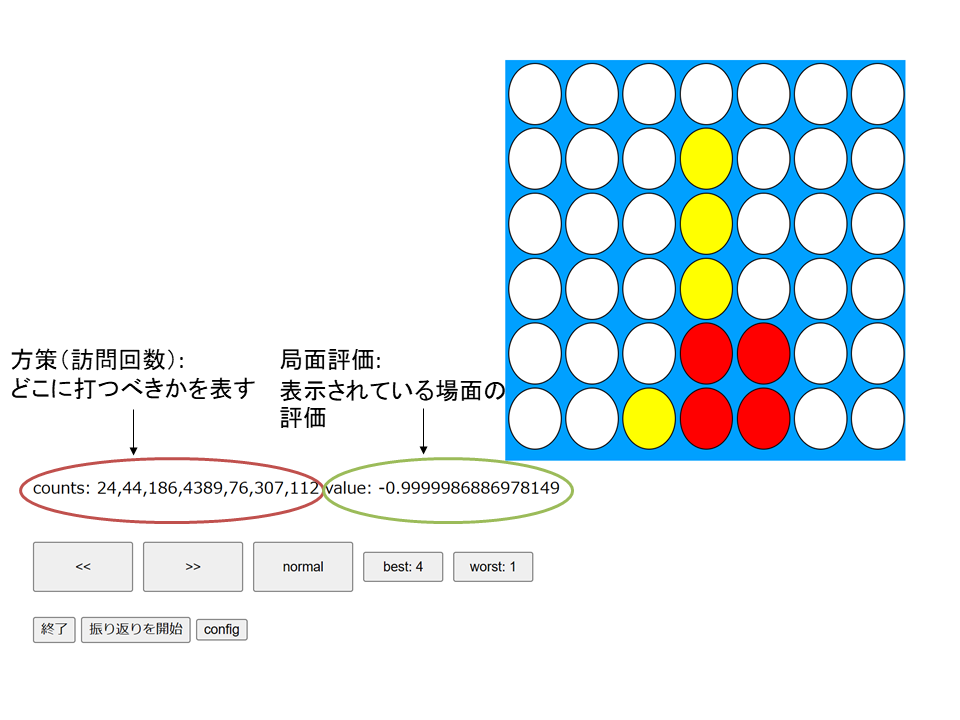
\includegraphics[width=\linewidth]{./figure/lookBack.png}
	\caption{振り返り画面}
	\label{fig:lookBack}
\end{figure}
数字が描かれたボタンは列のインデックスを表しており、各ボタンを押した際にその列を選択した場合の想定図と局面評価を確認できる。
\begin{figure}[t]
    \centering
    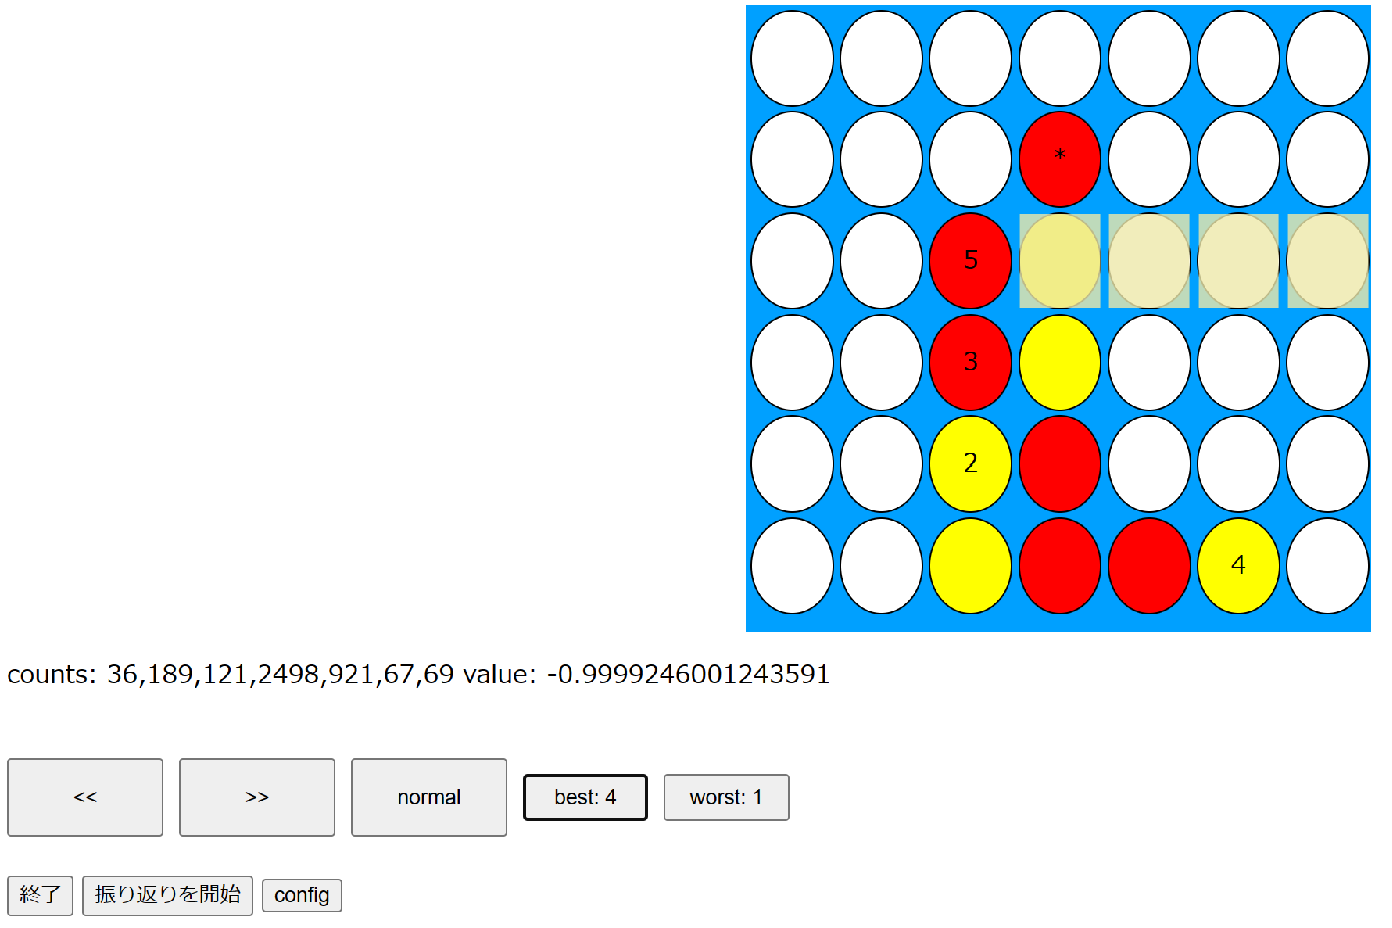
\includegraphics[width=\linewidth]{./figure/trajSystem.pdf}
	\caption{進行図の表示}
	\label{fig:trajSystem}
\end{figure}
\subsection{評価指標}
システム実験の評価指標は主観評価と客観評価の二つに分けられる。
主観評価は被験者による五段階評価であり、「タスクの熟達度に関連する質問」((a))と「タスクの楽しさ・面白さに関連する質問」((b))の二つに分けられる。
具体的な質問事項は付録Dに記載する。
客観評価はグループA(提案手法)の被験者とグループB(比較手法)の被験者の対戦成績である。

\subsection{実験結果}
進行図で提示される先読みの手数ごとに主観評価の平均値($1\sim5$)を表\ref{table:system-3}に示す。
先読みの手数は${3, 5, 7, \textrm{制限なし}}$の四種類であり、先読みの手数ごとに図\ref{fig:see}に示すように提示される進行図中の手数が変化する。
先読みの手数に関わらず、AIが予測する進行において最終的に4つ以上の石が並ぶ座標は強調表示される。
\begin{figure}[t]
    \centering
    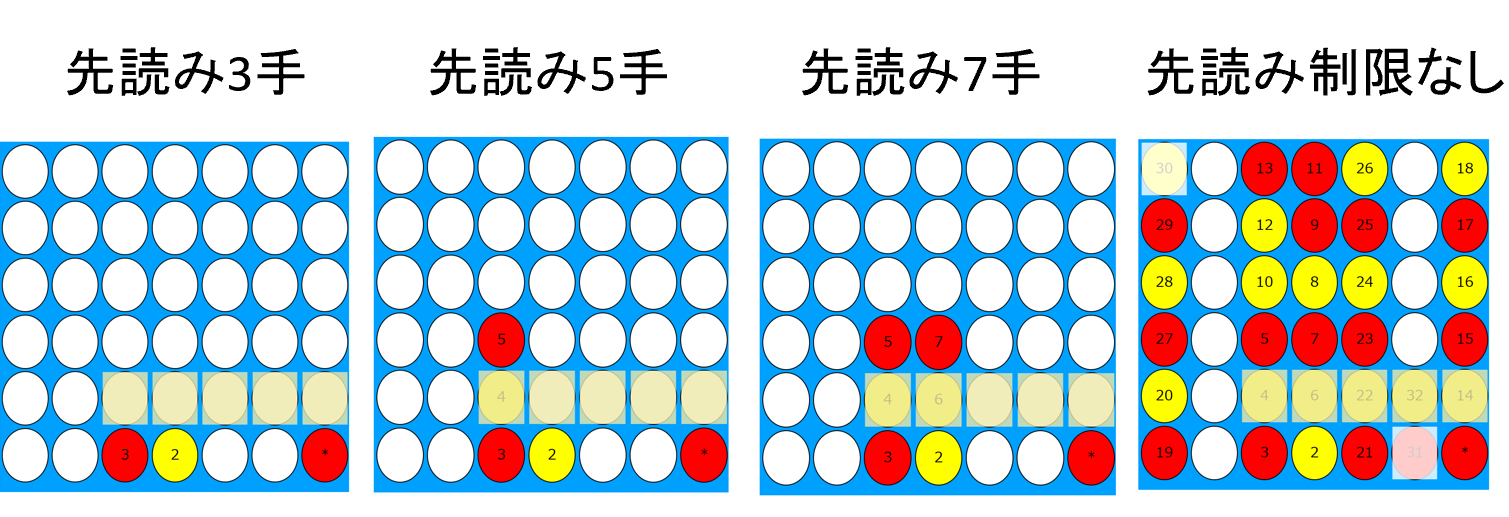
\includegraphics[width=\linewidth]{./figure/see.png}
	\caption{進行図の表示}
	\label{fig:see}
\end{figure}
先読み手数が3手または先読み手数制限なしの場合に、提案手法は比較手法に対して高い結果を示した。
\begin{table}[H]
    \caption{先読み手数3手の場合}
    \scriptsize
    \centering
    \resizebox{\linewidth}{!}{
        \begin{tabular}{c|l||c|c}
            \multicolumn{2}{c}{質問} & \multicolumn{2}{c}{主観評価} \\ \hline \hline
            質問の種類 & 質問の内容 & A & B \\ \hline 
            (a) & 振り返りによって成長したと感じましたか & \bf{3.29} & 3.17 \\
            & 振り返りによってAIの意図を掴むことができたと感じますか & 2.43 & \bf{2.67} \\
            & (二回目のみ) 一回目に比べて成長したと感じますか & 2.75 & \bf{4.33} \\ \hline
            (b) & 今後も connect4 をプレイするときにこのシステムを使いたいと思いましたか & \bf{3.71} & 3.67 \\
            & システムにより振り返りが楽しくなったと感じますか & {3.57} & \bf{3.60} \\
        \end{tabular}
    }
    \label{table:system-3}
\end{table}
\begin{table}[H]
    \caption{先読み手数5手の場合}
    \scriptsize
    \centering
    \resizebox{\linewidth}{!}{
        \begin{tabular}{c|l||c|c}
            \multicolumn{2}{c}{質問} & \multicolumn{2}{c}{主観評価} \\ \hline \hline
            質問の種類 & 質問の内容 & A & B \\ \hline 
            (a) & 振り返りによって成長したと感じましたか & 3.00 & \bf{4.00} \\
            & 振り返りによってAIの意図を掴むことができたと感じますか & 2.60 & \bf{4.00} \\
            & (二回目のみ) 一回目に比べて成長したと感じますか & 3.67 & \bf{4.33} \\ \hline
            (b) & 今後も connect4 をプレイするときにこのシステムを使いたいと思いましたか & 4.00 & \bf{4.80} \\
            & システムにより振り返りが楽しくなったと感じますか & 4.20 & \bf{4.60} \\
        \end{tabular}
    }
    \label{table:system-5}
\end{table}
\begin{table}[H]
    \caption{先読み手数7手の場合}
    \scriptsize
    \centering
    \resizebox{\linewidth}{!}{
        \begin{tabular}{c|l||c|c}
            \multicolumn{2}{c}{質問} & \multicolumn{2}{c}{主観評価} \\ \hline \hline
            質問の種類 & 質問の内容 & A & B \\ \hline 
            (a) & 振り返りによって成長したと感じましたか & {3.83} & \bf{4.33} \\
            & 振り返りによってAIの意図を掴むことができたと感じますか & 2.67 & \bf{3.67} \\
            & (二回目のみ) 一回目に比べて成長したと感じますか & 2.75 & \bf{4.33} \\ \hline
            (b) & 今後も connect4 をプレイするときにこのシステムを使いたいと思いましたか & 4.17 & \bf{4.67} \\
            & システムにより振り返りが楽しくなったと感じますか & 3.00 & \bf{3.50} \\
        \end{tabular}
    }
    \label{table:system-7}
\end{table}
\begin{table}[H]
    \caption{先読み手数制限なしの場合}
    \scriptsize
    \centering
    \resizebox{\linewidth}{!}{
        \begin{tabular}{c|l||c|c}
            \multicolumn{2}{c}{質問} & \multicolumn{2}{c}{主観評価} \\ \hline \hline
            質問の種類 & 質問の内容 & A & B \\ \hline 
            (a) & 振り返りによって成長したと感じましたか & \bf{4.25} & 4.00 \\
            & 振り返りによってAIの意図を掴むことができたと感じますか & \bf{3.50} & 3.00 \\
            & (二回目のみ) 一回目に比べて成長したと感じますか & 2.75 & \bf{4.33} \\ \hline
            (b) & 今後も connect4 をプレイするときにこのシステムを使いたいと思いましたか & \bf{4.5} & 4.00 \\
            & システムにより振り返りが楽しくなったと感じますか & \bf{4.75} & 4.40 \\
        \end{tabular}
    }
    \label{table:system-100}
\end{table}
また、第二段階である被験者同士の対戦結果を表\ref{table:result-battle}に示す。
付録Dに示すように被験者一人に対して二回対戦を行った。結果として示すscoreは勝利を1,敗北を-1,引き分けを0
とした二回の対戦の平均値として定義される。
結果は表\ref{table:result-battle}に記載する。提案手法を用いて訓練を行ったグループ(A)は比較手法を用いて訓練を行ったグループ(B)よりも高い
勝率を記録した。
\begin{table}[H]
	\caption{対戦の結果}
    \label{table:result-battle}
	\centering
	\scalebox{0.98}[0.98]{
		\begin{tabular}{c|c}
			グループ & score \\ \hline
			A(提案手法)    & \bf{0.25} \\ 
			B(比較手法)    & -0.15 \\
		\end{tabular}
	}
	
\end{table}
また、第三章で示した新たな重要度の定義(式\ref{new-imp})の妥当性を検証するため、盤面$s$の重要度$I(s)$と被験者が$s$の進行図を
見た時間$t$の相関を調査した。比較手法には式\ref{imp}の定義を用いた。
結果を表\ref{table:result-imp}に示す。いずれの手法も$t$との有意な相関が見られなかった。
\begin{table}[H]
	\caption{重要度と$t$の相関}
    \label{table:result-imp}
	\centering
	\scalebox{0.98}[0.98]{
		\begin{tabular}{c|c|c}
			日数& 提案手法 & 比較手法 \\ \hline
			1日目& {-0.035}& \bf{-0.034}\\
            2日目& {-0.083}& \bf{0.067}\\
		\end{tabular}
	}
	
\end{table}


\subsection{考察(システム実験)}


提案手法を用いたグループAがグループBを上回る評価を得たのは、主に先読みが最も短い3手の場合と最も長い制限なしの場合となった。

先読み3手・制限なしの場合のデータをさらに1日目、2日目で分類した結果、
\begin{itemize}
    \item 先読み3手の場合は1日目
    \item 先読み制限なしの場合は2日目
\end{itemize}

の方がよりグループAからの評価が高いことが分かった。
付録\ref{chap:system}で述べるように、1日目と2日目ではGUIの設定に差があり
1日目のGUIでは全ての選択肢(最大7種)を起点とした進行図を閲覧可能であるのに対し、2日目のGUIでは起点となる選択肢を
二つに制限した。
そのため、2日目は被験者が見られる進行図の数が1日目の約$\frac{1}{3}$となる。

そのため、「1日目・先読み3手の場合」と「2日目・先読み制限なし」の場合に被験者が受け取る情報量は近しいと推測される。

また、データを「被験者のグループ・日にち・先読み手数」によって分類し、「振り返りによってAIの意図を掴むことができたと感じますか」という質問に対する評価(以下把握満足度と表記)の降順に
並べ直した結果を表\ref{table:order}に示す。
\begin{table}[H]
	\caption{把握満足度}
    \label{table:order}
    \scriptsize
	\centering
	\scalebox{0.98}[0.98]{
		\begin{tabular}{c|c|c||c}
			グループ& 日 & 先読み手数 &把握満足度 \\ \hline
			B & 2 & 5 & 4.67\\
            B & 2 & 7 & 4.00\\
            A & 1 & 制限なし& 3.50\\
            A & 2 & 制限なし& 3.50\\
            B & 1 & 3& 3.50\\
            B & 1 & 制限なし& 3.33\\
            A & 1 & 3& 3.33\\
            \multicolumn{4}{c}{(\ldots)}\\
            A & 2 & 3 & 1.75\\
            B & 1 & 3 & 1.50\\

		\end{tabular}
	}
	
\end{table}

グループAのデータを日にちと先読み手数で分けた場合最も把握満足度が高いのは
「2日目・先読み制限なし」、次いで「1日目・先読み制限なし」、「1日目・先読み3手」となった。
最も情報が少ない「2日目・3手」はグループAの全8パターン中最下位となった。\\


グループBに対しても同様に「振り返りによってAIの意図を掴むことができたと感じますか」への評価を集計した結果、
最も評価が高いのは「2日目・5手」、次いで「2日目・7手」、「1日目・3手」となった。\\



また、付録\ref{chap:data}の表\ref{table:tail}より提案手法が示す1組の状態$s$、行動$a$について示す分岐の数$n$の平均は約10であるため、比較手法が示す情報量は提案手法の約$\frac{1}{10}$となる。
また、先読みの手数に制限が無い場合の手数の平均は約15手である。
そのため提示する情報量が大きい程評価が高くなるわけではなく、手法ごとに被験者が適切と感じる情報量が存在すると推測される。\\

以上の考察
を踏まえて、被験者に対して提示する情報を最小化した上で適切な情報量を調査するため、
先読みを1$\sim$5手として再実験を行った。
システム実験では補助として提示した訪問回数、局面評価に注目する被験者が多く見られたため、訪問回数「count」(訪問回数)の表示を廃止し、「value」(局面評価)と進行図の閲覧は被験者の手番(先番)となる盤面でのみ可能とした。

結果は以下のようになった。

(ここに表を入れる)


把握満足度と「充分な情報量」の平均は提案手法の方が高くなった。そのため、被験者が比較手法では情報量が不充分であると感じている
際に、提案手法で情報を補足することには一定の意義があると推測される。
また、先読みが1手や2手の場合は、提案手法による軌道が枝分かれせず、結果的に表示される軌道の数が小さくなる。
そのため、提案手法と比較手法の差異は「決定木中のどの部分を取り出すか」の差異となる。
付録\ref{chap:alg}の\ref{sec:fix}で述べたように提案手法で示す進行図は盤面の局面評価と符合するように調整されていることも評価に寄与したと
考えられる。
\chapter{結論}

本論文では
\begin{itemize}
	\item 決定木から有力なノードを抽出
	\item 収集されたノードのさらなるグループ化
	\item 決定木中の有力なノードへの過程の保存と提示
\end{itemize}

により,強化学習AIシステムの判断の可視化を試みた.
提案手法の有効性を示すため,connect4(ボードゲーム)を題材として2つの実験を行った.
第1の実験ではAI同士の対戦データを用いた提案手法の予測の妥当性を評価し,実際に比較手法よりも指標によっては優れた予測精度を示した.
第2の実験では自作のGUIシステムを用いた提案手法の有用性を検証し,ユーザーに提示される情報量が極端に大きい場合または小さい場合に比較手法よりも高いユーザー評価
を得うることがわかった.

課題としては,第4章において提案手法をconnect4に適用する際に「石を4つ並べたプレイヤーが勝利する」というゲームのルールに基づき
「4つ並んだ石の座標」を用いてノードのグループ化を行っていることが挙げられる.
この事はアルゴリズムの一部でドメイン知識を用いている事を意味し,さらなる汎用化の余地が存在する.
また,インタフェースとしてもユーザーに提示する情報の量や種類もさらなる調査の必要性を感じた.
そのため,
今後は
\begin{itemize}
	\item 手法のゲーム固有の知識(ドメイン知識)からの脱却
	\item ユーザーの学習支援に適切な情報提示の方式の模索
\end{itemize}


に取り組みたい.

\chapter*{謝辞}
\addcontentsline{toc}{chapter}{謝辞}
本研究を行うにあたり親身に相談に乗っていただき,ご指導してくださった萩原将文教授,
ならびに共に問題解決,議論,相談,および実験に付き合ってくださった研究室の先輩方,同期の皆様,
実験に参加してくださった大学の友人達に深く感謝いたします.
誠にありがとうございました.

% \addcontentsline{toc}{chapter}{参考文献}
\newpage
\pagestyle{fancyplain}\lfoot{}\cfoot{\thepage}\rhead{}
\lhead{\small \gt 参考文献~~}\chead{} \rhead{}
\addcontentsline{toc}{chapter}{参考文献}
\printbibliography[title=参考文献]

\appendix

% 付録はa, b, c,と見出しを付けていく
\chapter{データ実験の詳細}
\label{chap:data}
\section{使用したモデルの詳細}
第三章で述べたとおり使用した対戦データは弱いAIを先番とし,強いAIを後手としている.
AIの強さは一手ごとの探索を行う時間(time),付録Cで述べる$C_{puct}$,ニューラルネットワークの訓練段階におけるエポック数の値によって調整した.
timeと$C_{puct}$,エポック数はいずれも値が大きい程モデルは強くなると考えられる.(エポック数については付録\ref{chap:baseline}を参照)
対戦データ生成時のパラメータは表\ref{table:param-battle}の幅からゲームごとにランダムな値を採用した.
これはパラメータの値を変化させることでゲームデータに多様性を持たせるためである.
\begin{table}[H]
	\caption{対戦データのパラメータ}
	\label{table:param-battle}
	\centering
	\scalebox{0.98}[0.98]{
		\begin{tabular}{c|c|c}
			モデル&強&弱\\ \hline
			time    & 3-5 & 0-2 \\ 
			$C_{puct}$ & 0.8-1   & 0-0.5 \\
			エポック数 & 200 & 1 \\

		\end{tabular}
	}
	\label{table:battle}
\end{table}

\section{対戦結果の詳細}
2000ゲームのうち1983ゲームは強いAI(後番)の勝利となった.
また,ゲームごとの手数は75\%のゲームが36手以内で終了している.
そのため,データ実験ではゲームの中盤と言える13$\sim$24手目のデータを使用した.
図\ref{fig:stepCum}にゲームの終了手数の累計グラフを示す.
\begin{figure}[t]
	\centering
	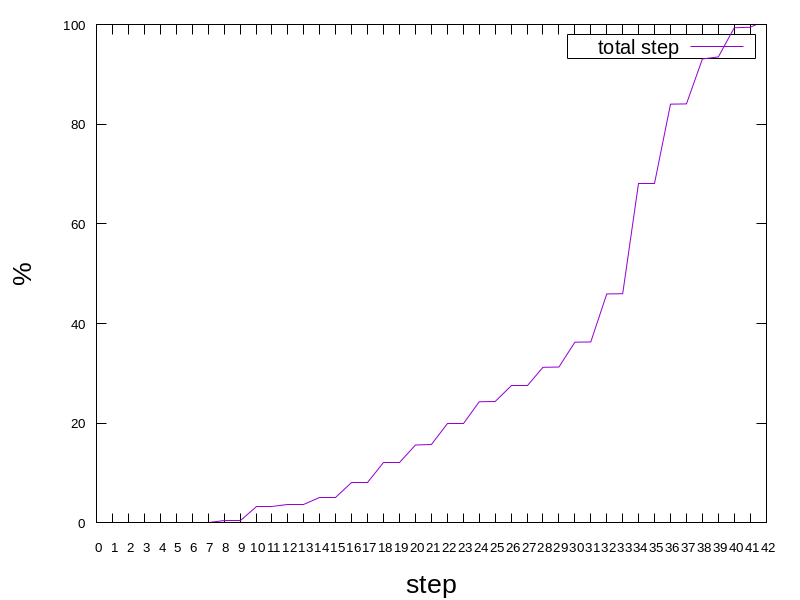
\includegraphics[width=\linewidth]{./figure/stepCum.png}
	\caption{終了手数の分布}
	\label{fig:stepCum}
\end{figure}
\section{評価指標の詳細}
本論文が提案する提案指標(group count, stone count)の計算において,盤面の座標は図\ref{fig:index}のように定められる.
\begin{figure}[t]
	\centering
	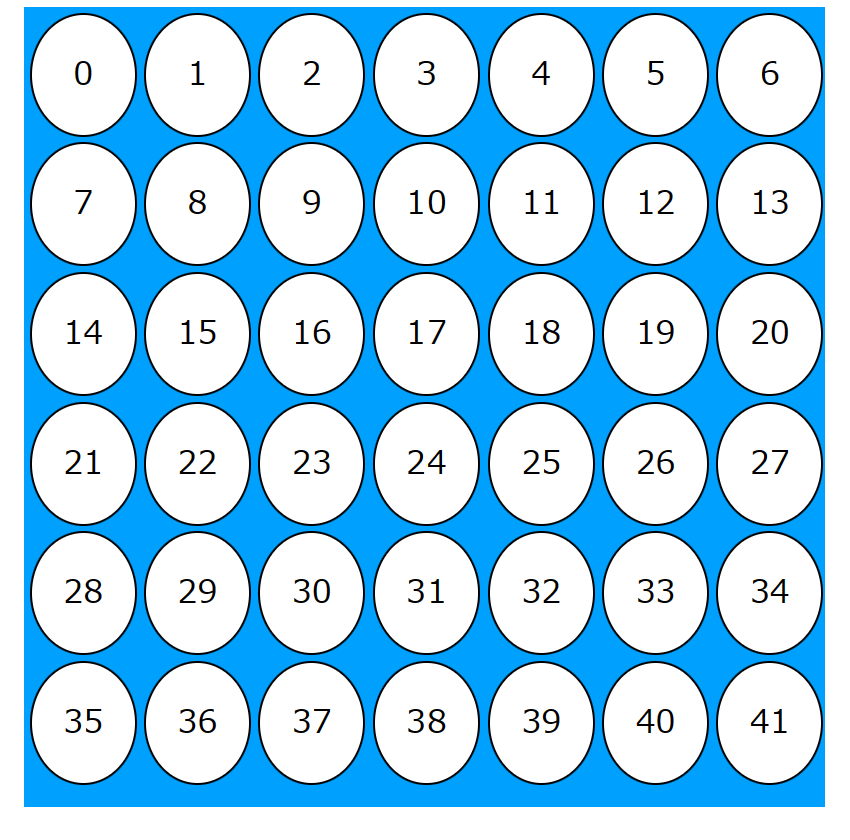
\includegraphics[width=100pt]{./figure/index.png}
	\caption{盤面の座標番号}
	\label{fig:index}
\end{figure}
ゲーム終了状態には図\ref{fig:fatalGroup}のように4つ以上連続してつながっている石の座標$F_s$(fatal stoneの集合)とその組み合わせ$F_g$(fatal groupの集合)を記録する.
下の図の盤面は$\{17, 18, 19, 20, 24, 31, 38\}$の7つのfatal stoneと$\{[17, 18, 19, 20], [17, 24, 31, 38]\}$の二つのfatal groupを持つ
\begin{figure}[t]
	\centering
	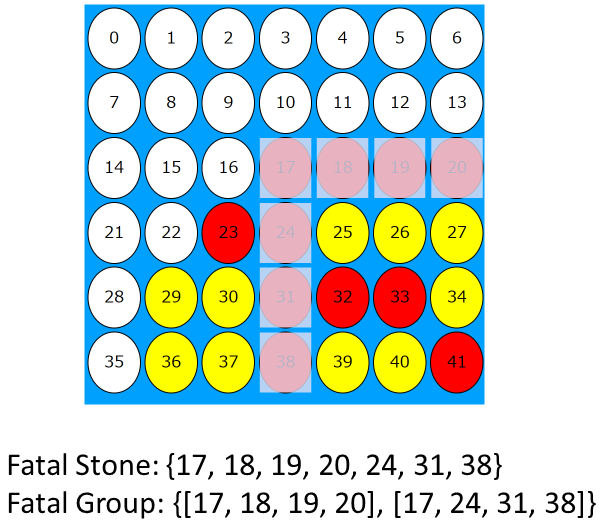
\includegraphics[width=\linewidth]{./figure/fatalGroup.png}
	\caption{fatalStoneとfatalGroup}
	\label{fig:fatalGroup}
\end{figure}
group count($C_g$), stone count($C_s$)は実際のゲームにおけるfatal groupとfatal stoneの集合(それぞれ$R_s, R_g$とする)とAIの予測によるfatal stoneとfatal groupの集合($F_g, F_s$)を比較する指標である.
どちらも値が高ければ高い程予測の精度が高いことを表す.
\subsection{group count}
fcountはfatal groupの精度を示す二値(0または1)の指標である.
\begin{equation}
	{C_g = 1 \quad \textrm{If} \quad F_g \cap R_g \ne \phi \quad \textrm{Else} \quad 0}
\end{equation}
例外として$R_g=\phi$(引き分け)の場合,$F_g$も空集合であるならばgroup countは1となる.
\subsection{stone count}
stone countはfatal stoneの精度を示す.stone countの値域は[0, 1]である.
(Count()は集合の要素数を数える関数)
\begin{equation}
	{\textrm{stone count} = \textrm{min}(\frac{\textrm{Count}(F_s \cap R_s)}{4}, 1)  }
\end{equation}
例外として$R_s=\phi$(引き分け)の場合,$F_s$も空集合であるならばstone countは1となる.
\section{データ実験における提案指標の計測}

\begin{enumerate}
	\item 比較手法: 決定木の走査によりたどり着いた$F_s, F_g$によってstone count, group countを計算した
	\item 提案手法: 第三章で述べたアルゴリズムによって収集された最終状態の集合$S=\{s_{edge_1}, s_{edge_2}, ..., s_{edge_{k^l}}\}$
	    を指標ごとにグループ化する.
		\begin{itemize}
			\item group count: fatal groupによって$S$をグループ化してできた集合$\{S_{g_1}, S_{g_2}, ..., S_{g_n}\}$($S_{g_i}$は組み合わせ$g_i$がfatal groupとなっている盤面の集合)
			を要素が多い順に二つ取り出す.抽出された二つの集合$\{S_{g_{m_1}}, S_{g_{m_2}}\}$における$\{g_{m_1}, g_{m_2}\}$で構成される集合を$F_g$とし,group countを計算した.
			\item stone count: $g_{m_1}$を$F_s$とし,stone countを計算した.
		\end{itemize}
		
\end{enumerate}

\section{データ実験に使用したモデルの詳細}
第4章に記載した表\ref{table:result-online}の結果を求める際に用いたモデルのパラメータを表\ref{table:param-data}に示す.
\begin{table}[H]
	\caption{データ実験:使用モデルのパラメータ}
	\centering
	\scalebox{0.98}[0.98]{
		\begin{tabular}{c|c}
			パラメータ名 & 値 \\ \hline
			time    & 対戦時の後番のモデルと同じ \\ 
			$C_{puct}$    & 対戦時の後番のモデルと同じ \\
			エポック数 & 200 \\
			$k$ (提案手法のみ)     & 4 \\
			$l$ (提案手法のみ)     & 2 \\
		\end{tabular}
	}
	\label{table:param-data}
\end{table}

表\ref{table:param-data}の通り,対戦データが生成された際のモデルのパラメータを使用している.
そのため本手法はモデルの構造とパラメータの値へのアクセスが可能な場合を想定したホワイトボックス的アプローチの実験であると言える.
モデルのtime, $C_{puct}$の値を固定して同様の手法を適用した場合の実験結果を\ref{sec:gray}で示す.
\section{末尾のグループ化}
提案手法は予想図とその予想図に至る分岐(両方を合わせて進行図と記載)を抽出する.
図\ref{fig:regroup}は分岐を末尾の3手で2つのグループに再編する様子を表している.(ここでは分岐は行動$a$の連続として表している)
\begin{figure}[t]
	\centering
	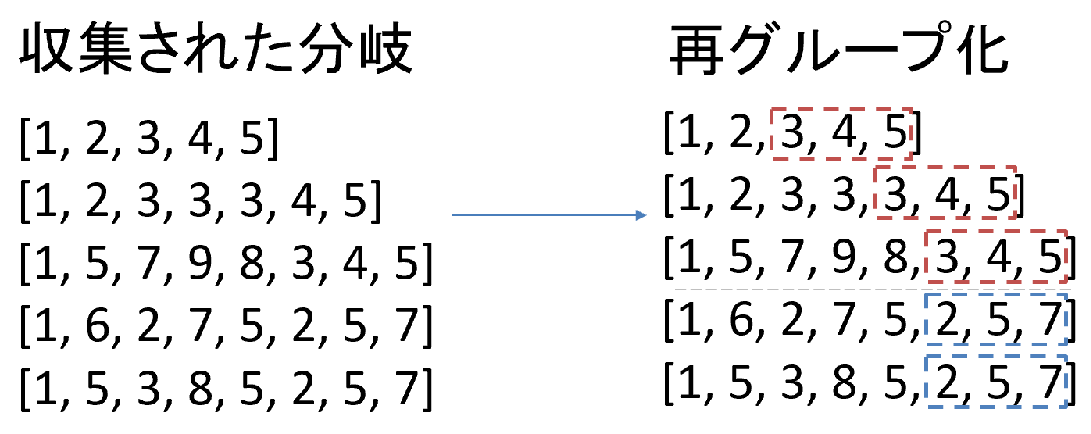
\includegraphics[width=\linewidth]{./figure/regroup.pdf}
	\caption{再グループ化}
	\label{fig:regroup}
\end{figure}
取り出された分岐を末尾の3手の選択でさらにグループ化した結果,元の分岐の数と再グループ化された分岐の数の平均は
表\ref{table:tail}のようになった.
結果として,取り出された分岐のうち,平均約2$\sim$3つの分岐において末尾の3手が共通する傾向にあることがわかった.
\begin{table}[H]
	\caption{再グループ化した際の分岐の数}
    \scriptsize
    \label{table:tail}
	\centering
	\scalebox{0.98}[0.98]{
		\begin{tabular}{c|c|c||c}
			手数(盤面数, 補間の有無)&  再グループ化前の分岐数(平均)&  再グループ化後の分岐数(平均)\\ \hline
			19-24(9862, 無)    &  & 0.44  \\
			19-24(9862, 有)    &  & 0.44   \\
			13-24(21022, 無)   & 6.95 & 3.08  \\
			13-24(21022, 有)   & 12.93 & 4.51 \\
		    0-40(61021,無)& 5.23 & 2.23\\
		    0-40(61021,有)& 10.82 & 3.78\\
		\end{tabular}
	}

	
\end{table}
また,各分岐の長さの平均は\ref{fig:length}のようになった.
尚,正確には1つの盤面,行動(最も訪問回数が大きい行動)の組に対して取り出される軌道の平均を更に平均した値を示している.
\begin{table}[H]
	\caption{分岐の長さの平均}
    \scriptsize
    \label{fig:length}
	\centering
	\scalebox{0.98}[0.98]{
		\begin{tabular}{c|c}
			手数(盤面数, 補間の有無)&  分岐の長さ(平均)\\ \hline
		    0-40(61021,無)& 10.89\\
		    0-40(61021,有)& 15.31\\
		\end{tabular}
	}	
\end{table}

\section{グレーボックス的手法}
\label{sec:gray}
モデルのパラメータを固定し,再び第四章のデータ実験を行った.パラメータの値を固定しているため,本実験はモデルの具体的なパラメータの値へのアクセスが不可能な場合にも適用可能な
グレーボックス的手法であると言える.
固定されたパラメータを表\ref{table:param-data-extra}に示す.
\begin{table}[H]
	\caption{データ実験(追加):使用モデルのパラメータ}
	\centering
	\scalebox{0.98}[0.98]{
		\begin{tabular}{c|c}
			パラメータ名 & 値 \\ \hline
			time    & 5 \\ 
			$C_{puct}$    & 1 \\
			エポック数 & 200 \\
			$k$ (提案手法のみ)     & 4 \\
			$l$ (提案手法のみ)     & 2 \\
		\end{tabular}
	}
	\label{table:param-data-extra}
\end{table}

実験の結果は表\ref{table:result-offline}のようになった.第四章に記載したホワイトボックス的手法と同様に提案手法はgroup countにおいて比較手法より高い値を示した.
\begin{table}[H]
	\caption{実験結果:データ実験}
	\centering
	\scalebox{0.98}[0.98]{
		\begin{tabular}{c|c|c|c|c}
			\multicolumn{1}{c}{} & \multicolumn{2}{|c|}{group count} 
			& \multicolumn{2}{c|}{stone count}\\ \hline \hline
			手数(盤面数, 補間の有無)    & 提案手法 & 比較手法 & 提案手法 & 比較手法 \\ \hline
			19-24(9862, 無)    & \bf{0.60} & 0.44 & 0.61 & \bf{0.63} \\
			19-24(9862, 有)    & \bf{0.63} & 0.44 & 0.61 & \bf{0.63}  \\
			13-24(21022, 無)   & \bf{0.53} & 0.37 & 0.55 & \bf{0.56}  \\
			13-24(21022, 有)   & \bf{0.55} & 0.37 & 0.55 & \bf{0.56}  \\
		\end{tabular}
	}
	\label{table:result-offline}
\end{table}

\chapter{各種アルゴリズムの詳細}
\section{比較手法のアルゴリズム}
比較手法の疑似コードを以下に示す。疑似コード中のTraverse()は第三章の疑似コード \ref{alg:myalg-1} \ref{alg:myalg-2}と同一である。
\begin{algorithm}
    \caption{比較手法のアルゴリズム}
    \begin{algorithmic}[1]       
        \State $t$: 手法を適用する探索木
        \State $T$: 状態遷移関数
        \State $\zeta(s, s')$: ノード$s$から$s'$までの軌道
        \Function{CompareAlgorithm}{$s, a$}
           \State $s_n \gets T(s, a)$
           \State $\zeta(s, s_n) \gets \{s, a, s_n\}$
           \State $\zeta \gets$ \Call{$s_n, \zeta(s, s_n)$}
           \Return $\zeta$
        \EndFunction
        
        \Function {Traverse}{$s, \zeta(s_{start}, s)$}
            \State $s_{now} \gets s$
            \State $\zeta_r \gets \zeta(s_{start}, s)$
            \While {$s_{now}が探索済みかつ終了状態でない$}
                \State $a_t \gets \textrm{argmax}_a N(s_{now}, a)$
                \State $s_n \gets T(s_{now}, a_t)$
                \State $\zeta_r.append({a_t, s_n})$
                \State $s_{now} \gets s_n$
            \EndWhile
            \Return $\zeta_r$
        \EndFunction
       
        
    \end{algorithmic}
\end{algorithm}


\section{提案手法におけるニューロ補間}
第四章におけるデータ実験、システム実験ではいずれも手法のニューラルネットワークによる補間を行っている。
第四章で示した疑似コードでは未探索のノードにたどり着いた際は走査を終了する。ニューラルネットワークによる補間とはこの場合、
方策$P(s, a)$で訪問回数$N(s, a)$を代用し走査を継続することである。
以下にニューロ補間を行う場合の疑似コードを示す(変更部分に下線)。
比較手法に対してニューロ補間を行う場合も同様にTraverse()のコードを変更する。
\begin{algorithm}
    \caption{提案手法のアルゴリズム(ニューロ補間あり)part1}
    \small
    \begin{algorithmic}[1]       
        \Function{CollectBoards}{$s, a, l, k$}
           \State $s_{now} \gets T(s, a)$
           \State $Z \gets $ empty queue
            \If{$s$が終了状態のとき}
             \Return  $Z$
            \EndIf
            \If{$s$が未探索のとき}
             \State \underline{方策$P(s)$から上位$k$の行動$\{a_1, a_2, ..., a_{k}\}(=\alpha)$を取り出す}
            \Else
             \State 訪問回数$N(s)$から上位$k$の行動$\{a_1, a_2, ..., a_{k}\}(=\alpha)$を取り出す
            \EndIf
           \For {each $a_i$ in $\alpha$}
             \State $s_{{next}_i} \gets T(s_{now}, a_i)$
             \State $\zeta(s_{now},s_{{next}_i})(=\{s_{now}, a_i, s_{{next}_i}\})$を$Z$の末尾に追加
           \EndFor
           \If{l=1}
             \Return $Z$
           \EndIf
           \State $i \gets 1$
           \While {$i < l$}
                \For {each $\zeta(s_{now}, s_{j})$ in $Z$}
                    \State $\zeta(s_{now}, s_{j})$ を $Z$からポップ
                    \If{$s$終了状態のとき}
                        \State $\zeta(s_{now}, s_{j})$ を$k$回$Z$の末尾に追加
                        \State continue
                    \EndIf
                    \If{$s$が未探索のとき}
                       \State \underline{方策$P(s)$から上位$k$の行動$\{a_1, a_2, ..., a_{k}\}(=\alpha)$を取り出す}
                   \Else
                    \State 訪問回数$N(s)$から上位$k$の行動$\{a_1, a_2, ..., a_{k}\}(=\alpha)$を取り出す
                   \EndIf
                    
                    \For {each $a_i$ in $\alpha$}
                        \State $s_{{next}_j} \gets T(s_{j}, a_i)$
                        \State $\zeta(s_{now},s_{{next}_i})(=\zeta(s_{now}, s_{j}).append({a_i, s_{{next}_i}}))$を$Z$の末尾に追加
                    \EndFor
                    
                \EndFor     
           \EndWhile
           \Return $Z(=\{\zeta(s_{start}, {s'}_1), ..., \zeta(s_{start}, {s'}_{k^l})\})$
        \EndFunction
    \end{algorithmic}
\end{algorithm}
\begin{algorithm}
    \caption{提案手法のアルゴリズム(ニューロ補間あり)part2}
    \begin{algorithmic}[1] 
        \Function {Traverse}{$s, \zeta(s_{start}, s)$}
        \State $s_{now} \gets s$
        \State $\zeta_r \gets \zeta(s_{start}, s)$
        \While {$s_{now}$が終了状態でない}
            \If{$s$が未探索のとき}
                \State \underline{$a_t \gets \textrm{argmax}_a P(s_{now}, a)$}
            \Else
                \State $a_t \gets \textrm{argmax}_a N(s_{now}, a)$
            \EndIf
            \State $s_n \gets T(s_{now}, a_t)$
            \State $\zeta_r.append({a_t, s_n})$
            \State $s_{now} \gets s_n$
        \EndWhile
        \Return $\zeta_r$
        \EndFunction
       
        
    \end{algorithmic}
\end{algorithm}
\section{システム実験における提案手法の変更}
システム実験では画面の左下に盤面$s$の訪問回数$N(s)$と局面評価$V(s, a)$を表示する。このとき
$V(s, a)$の絶対値(どちらのプレイヤーの勝利に近いか)と予想図の勝敗が異なる場合、ユーザーの混乱を招く可能性がある。
そのため、提案手法では勝敗が$V(s, a)$の絶対値と一致する軌道を表示するように修正を施した。
システム実験用に修正された疑似コードはAlgorithm:\ref{alg:system}となる。(下線が変更部分)
また、提案手法により収集した最終盤面$S=\{s_{edge_1}, s_{edge_2}, ..., s_{edge_{k^l}}\}$は
最終的に4つ以上連続してつながっている石の組み合わせ(fatal group)でグループ化し、最も要素数が多い集合の道筋をユーザーに提示した。

\begin{algorithm}
    \caption{提案手法のアルゴリズム(システム実験)}
    \label{alg:system}
    \begin{algorithmic}[1]       
        
        \Function {Traverse}{$s, \zeta(s_{start}, s)$}
        \State  \underline{$\zeta(s_{start}, s)$から$s_{start}$の次の行動$a$を取り出す}
        \State \underline{$v \gets V(s, a)$}
        \State $s_{now} \gets s$
        \State $\zeta_r \gets \zeta(s_{start}, s)$
        \While {$s_{now}$が終了状態でない}
            \If{$s$が未探索のとき}
                \State \underline{$a_t \gets \textrm{argmax}_a P(s_{now}, a)$}
            \Else
                \State $a_t \gets \textrm{argmax}_a N(s_{now}, a)$
            \EndIf
            \State $s_n \gets T(s_{now}, a_t)$
            \State $\zeta_r.append({a_t, s_n})$
            \State $s_{now} \gets s_n$
        \EndWhile
        \If{\underline{$v$と$V(s_{now})$の絶対値が異なるとき}}
           \Return null
        \EndIf
        \Return $\zeta_r$
        \EndFunction
       
        
    \end{algorithmic}
\end{algorithm}

\chapter{alphazero\_baseline}
\label{chap:baseline}
\section{ニューラルネットワーク}
モデルの構成を図\ref{fig:baselineNetwork}に示す.
alphazero\_baselineにおける選択肢は列の数と等しい7であるため,1$\times$7の行列となる.
例えば方策が
$\left\{0, 0.1, 0.2, 0, 0, 0.7, 0.8\right\}$であるとき,方策中の最も大きい成分は7番目の0.8であるため,プレイヤーは次に7列目を選択する事が推奨される.
\begin{figure}[t]
	\centering
	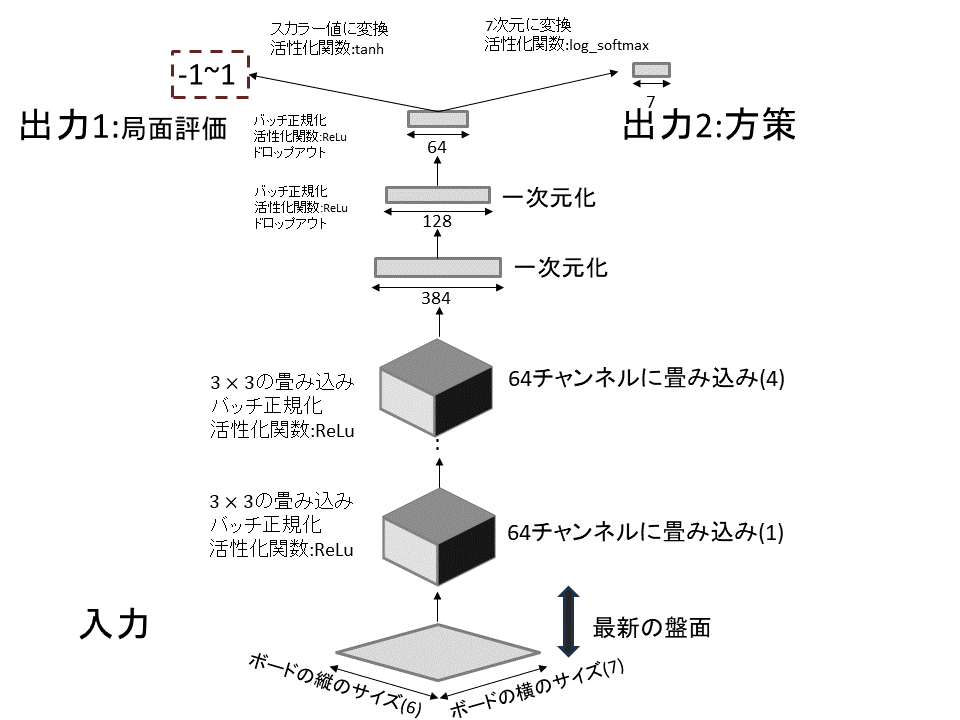
\includegraphics[width=\linewidth]{./figure/baselineNetwork.png}
	\caption{alphazero\_baselineネットワークの構成}
	\label{fig:baselineNetwork}
\end{figure}
また,モデルの訓練過程は以下のステップをまとめて1エポックとした繰り返しによって構成されている.
使用したテストデータ\cite{dataset}はα-β木探索によるconnect4の解から生成されている\cite{scoring}.
\begin{enumerate}
	\item 500ゲーム分の自己対戦を行う
	\item 自己対戦によって収集した盤面を入力としてネットワークを訓練
    \item ネットワークを教師データによって評価
    \item 新しいネットワークを用いたAIと訓練前の最善のネットワークを用いたAIによる対戦を50ゲーム分行い6割以上
    の勝率を記録した場合,新しいネットワーク最善のネットワークとして保存する

\end{enumerate}
本論文の第3章におけるシステム実験で用いた「強いAI」のニューラルネットワークは上記をステップを200エポック分実行して訓練されたモデルを使用している.

また,ネットワーク訓練時のパラメータの値を\ref{table:param-train}に示す.
\begin{table}[H]
	\caption{ネットワーク訓練時のパラメータ名と値}
	\centering
	\scalebox{0.98}[0.98]{
		\begin{tabular}{c|c}
			パラメータ名 & 値 \\ \hline
			学習率(lr)    & 0.001 \\ 
			dropout    & 0.3 \\
			epochs      & 5 \\
			batch\_size     & 64 \\
			num\_channels  & 64 \\
		\end{tabular}
	}
	\label{table:param-train}
\end{table}
\section{alphazero\_baselineのパラメータ更新}
alphazero\_baselineのパラメータ更新は第2章で述べた手順とほぼ同一であるがPUCTスコア$U(s, a)$の定義と$Q(s, a)$の更新則に差異がある.
$ C_{\textrm{cpuct}}$はハイパーパラメータである.
($N(s), N(s, a)はそれぞれs,(s, a)に対して探索を行った回数$)
\begin{equation}
	{U(s, a)= C_{\textrm{cpuct}}P(s, a)\frac{\sqrt{N(s)}}{1+N(s, a)}\\
	}
\end{equation}

$Q(s, a)$は以下のように更新される.
($s_cは現在の探索ノードsから見た最もPUCTスコアU(s, a)とQ(s, a)の和の高い子ノード$)
\begin{equation}
	{Q(s, a)=\frac{N(s, a)Q(s, a)+V(s_c)}{N(s, a)+1}\\
	}
\end{equation}
これらの変更を加えたalphazero\_baselineにおけるPV-MCTSのアルゴリズムをAlgorithm\ref{alg:base}に示す.
\newpage

\begin{algorithm}
    \caption{PV-MCTS in alphazero-baseline (変更部分)}
    \label{alg:base}
    \begin{algorithmic}[1]
    \small
        \State $t$: 決定木
        \State $T$: 遷移関数
        \State $N(s, a)$: $(s, a)$の組み合わせを探索した回数
        \State $Q(s, a)$: 行動価値関数 ($\textrm{Explore}(s)$の平均)
        \State $W(s, a)$: 行動価値の総和$(W(s, a)=Q(s, a)N(s, a))$
        \State $P(s, a)(=P(s_n), s_n=T(s, a))$: 
        \State ニューラルネットワークから出力された方策
        \State $V(s, a)(=V(s_n), s_n=T(s, a))$: 
        \State ニューラルネットワークから出力された局面評価
        \Function{TreePolicy}{$s$}
            \If {$s$が探索されていない子ノードを持つとき}
                \State $s_c \gets T(s, a)$ ($s_c$は未探索のノード)
                \State \Call{InitNode}{$s_c$}
                \State \Return $a$
            \Else
                \State 以下のPUCTスコア$U(s, a)$を計算
                \State \underline{$U(s, a)= C_{\textrm{cpuct}}P(s, a)\frac{\sqrt{N(s)}}{1+N(s, a)}$}
                \State $(N(s)=\Gamma N(s, a))$
                \State 以下のように$a$を求める
                \State $a = {\textrm{argmax}}_a (Q(s, a)+U(s, a))$
                \State \Return $a$
                
            \EndIf
        \EndFunction
        \Function{Backpropagate}{$\zeta, G$}
            \For {each node-action pair $(s, a)$ in $\zeta$}
                \State $N(s, a) \gets 0$
                \State $W(s, a) \gets 0$
                \State $Q(s, a) \gets 0$
            \EndFor
        \EndFunction
        \Function{InitNode}{$s$}
            \For {each action $a$ from  $s$}
                \State $N(s, a) \gets N(s, a)+1$
                \State $W(s, a) \gets W(s, a)+G$
                \State \underline{$Q(s, a) \gets \frac{N(s, a)Q(s, a)+V(s_c)}{N(s, a)+1}$}
				\State $(s_c = T(s, a))$
            \EndFor
        \EndFunction
    \end{algorithmic}
\end{algorithm}
\chapter{インタフェース実験の詳細}
\label{chap:system}
インタフェース実験では全3回にわたる実験を行い,被験者同士の対戦を行う第3回以外の2回は被験者がAIとの対戦とAIを用いた振り返りを行う.
第4章と同様に3回セットの実験のうち,1回目と2回目を第1段階、3回目を第2段階と呼ぶ.
以下で被験者のデータの詳細を述べ,それから実験設定や結果の詳細を段階ごとに述べていく.
\section{被験者のデータ}
実験対象者は計22人の10代-20代学生(男性17名:女性5名)であり,表\ref{table:before}に示す各種の事前質問($1\sim5$の値で答える)の結果は以下となった.
ボードゲームの経験を問う質問に関しては1を「1年に1回程プレイする」程度,5を「週に2,3回以上プレイする」程度と定めた.
connect4の経験を問う質問に関しては1を「connect4を知らない」程度,5を「週に2,3回以上プレイする」程度と定めた.
また,機械学習と強化学習の知識を問う質問に関しては1を「言葉を聞いたことがある」程度,5を「機械学習についての入門書を読んだり,授業を受けたことがある」程度と定めた.
また,被験者には先述のAllis\cite{allis}による9strategyをはじめとしたconnect4の知識的解法をネット検索等の手段で調べないよう要請した.
\begin{table}[H]
    \caption{事前質問項目:インタフェース実験}
    \label{table:before}
	\small
    \begin{tabular}{c||c}
        \multicolumn{1}{c}{質問} & 回答の平均\\ \hline \hline
        ボードゲームの経験はどれくらいありますか & 2.18\\
        connect4(ゲーム)の経験はどれくらいありますか& 1.64\\\hline
        機械学習に対する知識はどれくらいありますか& 3.59\\
        強化学習に対する知識はどれくらいありますか& 3.23\\
    \end{tabular}
    
\end{table}
\section{第1段階}
第1段階はAIとの対戦とその振り返りによって構成されている.
振り返りモードでは表示する進行図の手数,AIの強さを被験者ごとに変更しつつ実験を行った.
進行図の手数は$\{3, 5, 7, 制限なし(最後まで表示)\}$の4段階,AIの強さは$\{強,弱\}$の2段階を設定した.
また,対戦を行うAIモデルを用いて振り返りの進行図を生成した.
使用したAIモデル(alphazero\_baseline),提案手法に与えるパラメータを表\ref{table:param-system}に示す.
\begin{table}[H]
	\caption{AIモデルのパラメータ(インタフェース実験第1段階)}
    \label{table:param-system}
	\centering
	\scalebox{0.98}[0.98]{
		\begin{tabular}{c|c|c}
			モデル&強&弱\\\hline
			time    & 5 & 1 \\ 
			$C_{puct}$ & 1   & 0.25 \\
            エポック数 & 200 & 1 \\
			$k$ (提案手法のみ)     & 4 & 4 \\
			$l$ (提案手法のみ)     & 2 & 2 \\

		\end{tabular}
	}
	
\end{table}
また,1回の実験当たりの制限時間は7分とし,実験内のAIとの対戦は2回までに制限した.
これは実戦経験による熟達ではなく支援システムによる学習過程の観察という実験の趣旨に従うためである.
\subsection{振り返りモード(GUI)の詳細}
振り返りモードでは直前の対戦の内容を振り返ることができる.
「>/<」ボタンを押すことで「1つ先の盤面に進む/戻る」ことができる.
また,振り返りを補助する機能として画面左下の「counts」に表示されている盤面$s$に対する
各行動の訪問回数$N(s)$,「value」に局面評価$V(s)$を示した.
$N(s),V(s)$は対戦に使用したモデルから導かれる.
数字が書かれているボタンはAIモデル(対戦に使ったモデルと同じ)による進行図を提示するボタンであり,ボタンに描かれた数字
と同じ列を選択した場合の進行図を見ることができる.
図\ref{fig:number-button}では「4」と描かれたボタンを押した結果,左から4番目を選択した場合の進行図が表示されていることがわかる.
選択した位置は「*」マークで表示される.



\begin{figure}[htbp]
    \centering
    \setlength{\fboxsep}{1pt} % フレームの余白を調整
    \setlength{\fboxrule}{1pt} % フレームの太さを調整
    \fbox{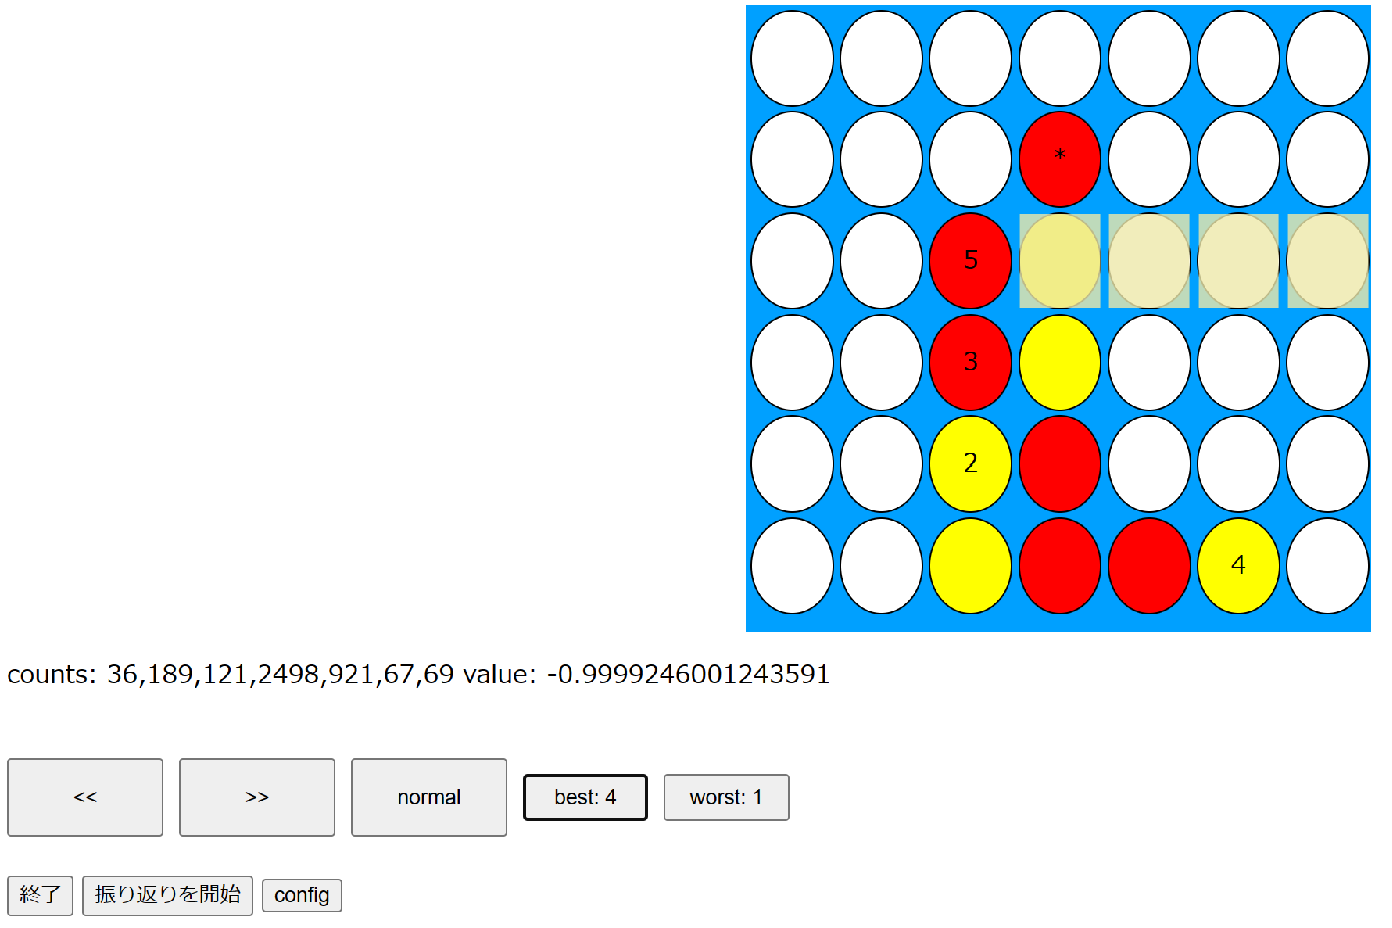
\includegraphics[width=\linewidth]{./figure/trajSystem.pdf}}
    \caption{進行図の提示}
	\label{fig:number-button}
\end{figure}
想定図中の数字は数字の大きさの順番に石が置かれるというAIの予想を表している.図\ref{fig:multi}
では赤が「*」マークの位置に石を置いた次に黄は左から3列目の位置,その次に赤は左から3列目に打つことが予測されている.
また,図中で色づけられている部分は進行図においてその部分がは4つ以上つながることを示している.赤く色づけられている場合はその部分で
赤が4つ以上つながると予想されていること,黄色く色づけられている場合はその部分で黄色が4つ以上つながると予想されているこを示している.
また,提案手法による振り返りが適用されたグループでは提示される進行図が複数となる.そのため図\ref{fig:multi}に示すように他の想定図を見ることができる「next\_prej/pre\_traj」
ボタンが追加される.
\begin{figure}[htbp]
	\centering
	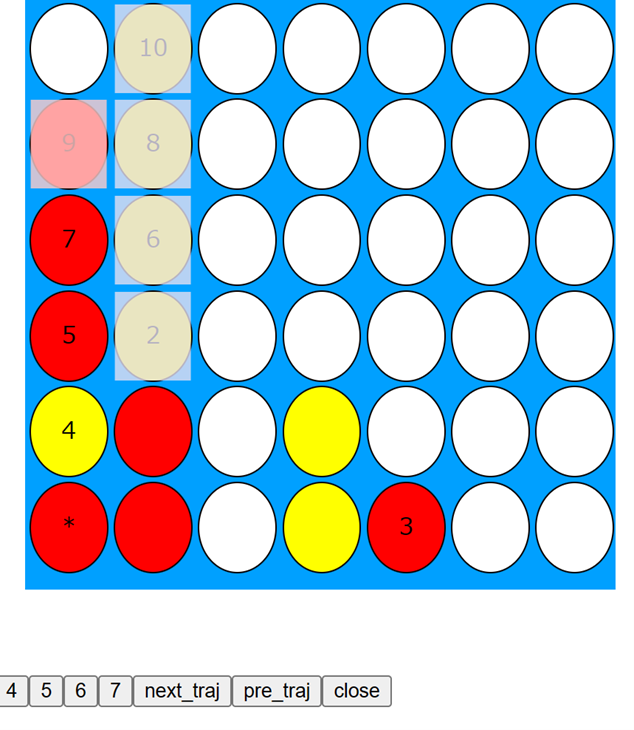
\includegraphics[width=150pt]{./figure/multi.png}
	\caption{提案手法による進行図の提示}
	\label{fig:multi}
\end{figure}
ここからは第1段階中の1日目,2日目のGUIの違いについて述べる.
\subsection{1日目}
1日目は被験者の操作間への慣れを促進するため全ての選択肢に対し進行図表示ボタン(数字ボタン)を設置した.
図\ref{fig:traj-button}に示すようにこれらのボタンは「traj」ボタンを押すことで出現する.

\begin{figure}[htbp]
    \centering
    \setlength{\fboxsep}{1pt} % フレームの余白を調整
    \setlength{\fboxrule}{1pt} % フレームの太さを調整
    \fbox{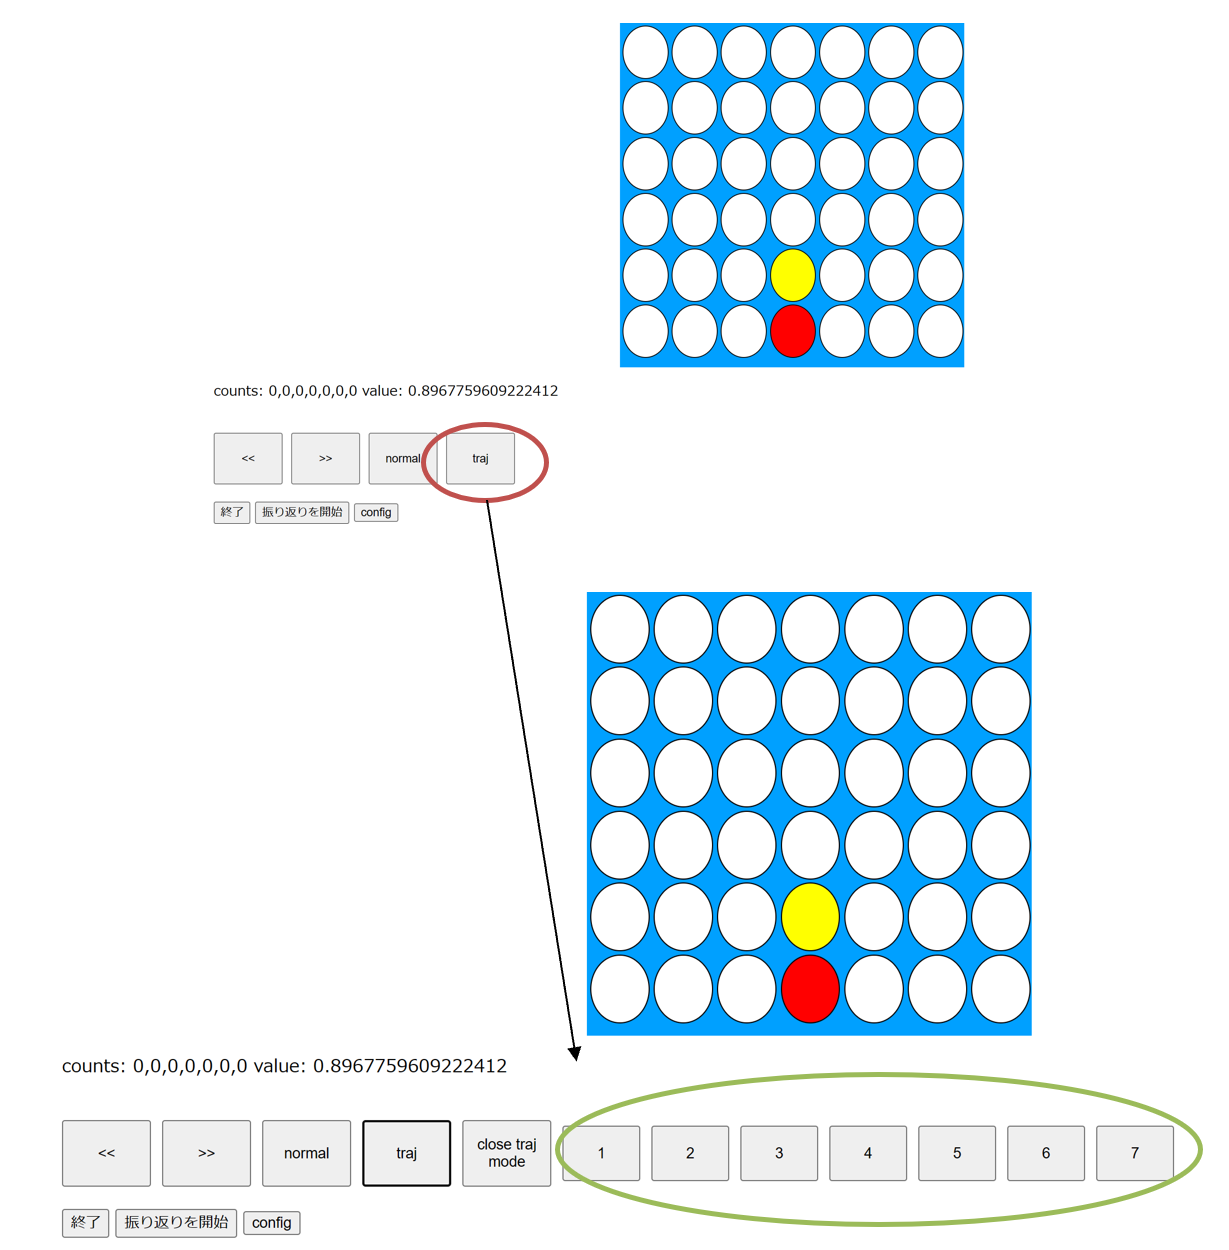
\includegraphics[width=\linewidth]{./figure/traj-button.png}}
    \caption{進行図表示ボタン(1日目)}
	\label{fig:traj-button}
\end{figure}

\subsection{2日目}
2日目は進行図の閲覧を促進するためtrajボタンを廃止し,最も訪問回数$N(s,a)$の多い選択肢$a_{max}$,少ない選択肢$a_{min}$
からの進行図を示すボタンをそれぞれ「best:(列の数字)」「worst:(列の数字)」のラベルで図\ref{fig:best-worst}のように表示した.

\begin{figure}[htbp]
    \centering
    \setlength{\fboxsep}{1pt} % フレームの余白を調整
    \setlength{\fboxrule}{1pt} % フレームの太さを調整
    \fbox{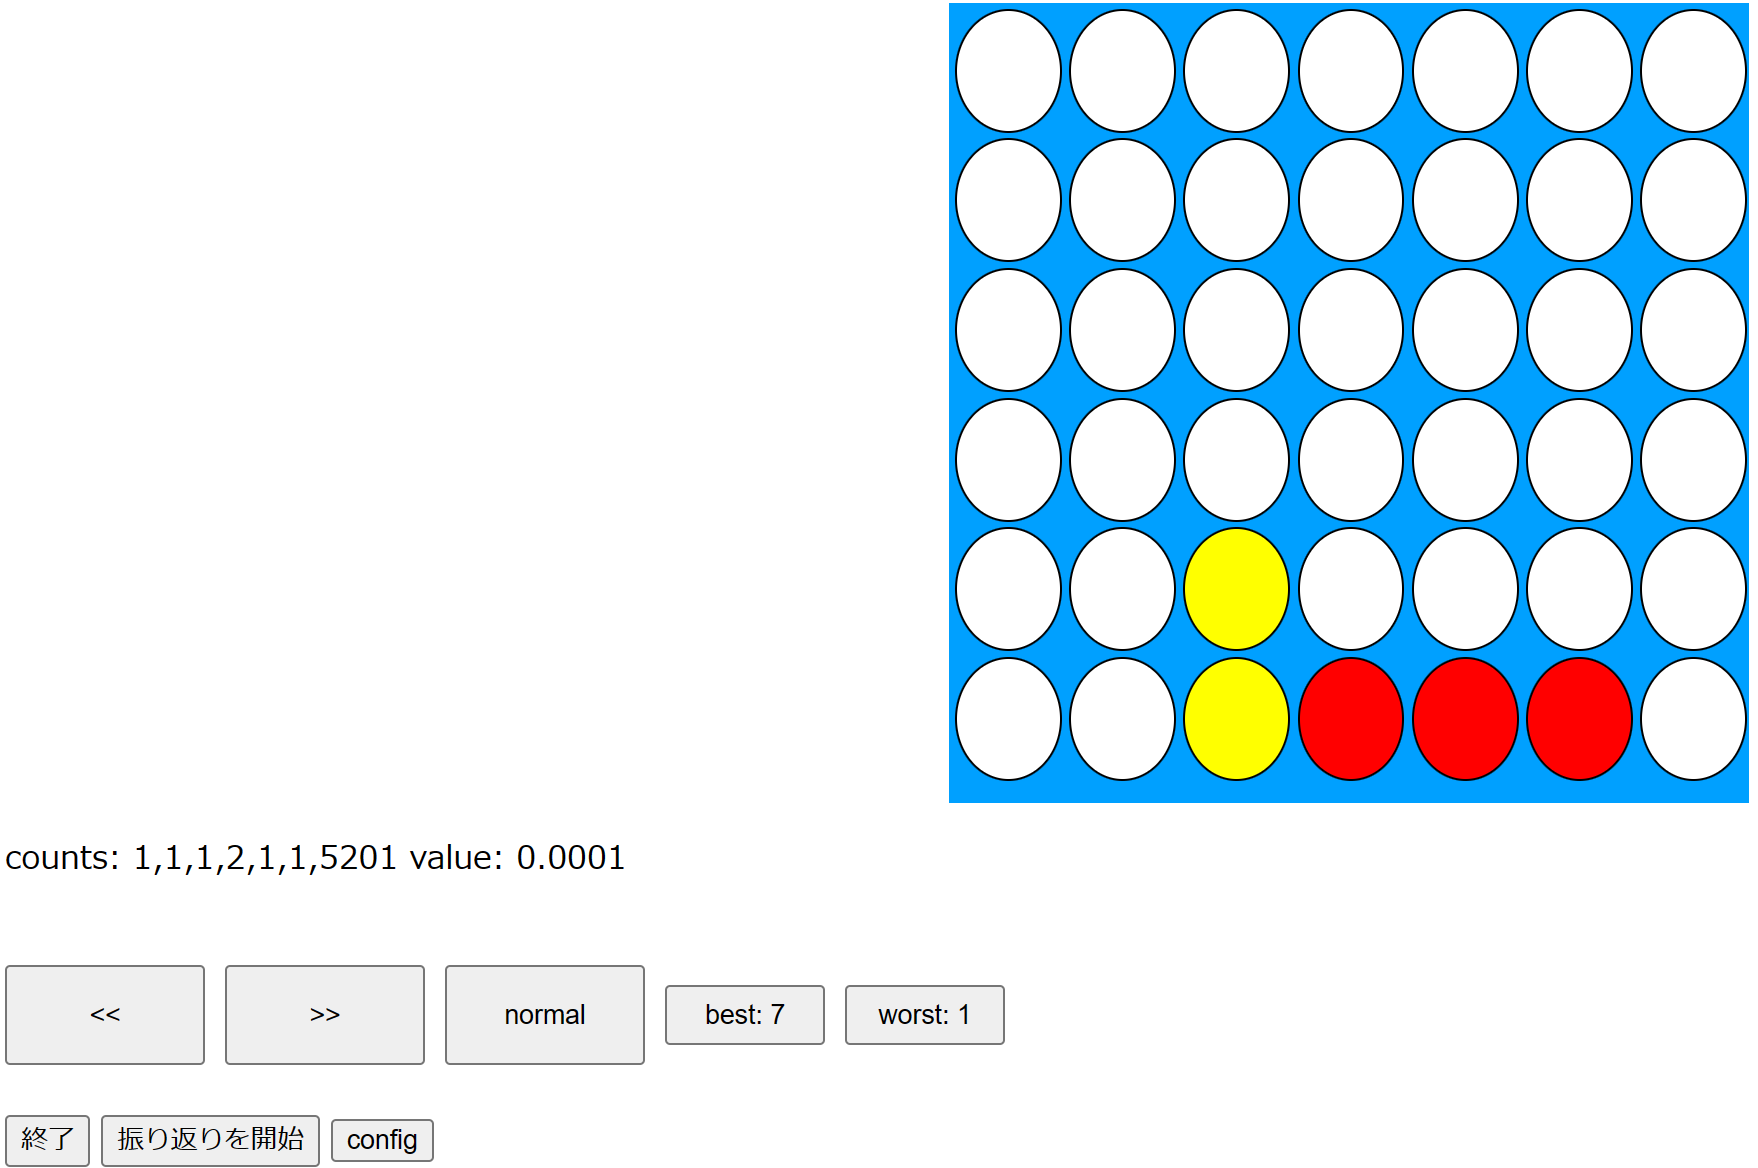
\includegraphics[width=\linewidth]{./figure/best-worst.png}}
    \caption{進行図表示ボタン(2日目)}
	\label{fig:best-worst}
\end{figure}

\section{第2段階}
第2段階は提案手法を用いて振り返りを行ったグループ(A)の被験者と比較手法を用いて振り返りを行ったグループ(B)の被験者の対戦である.
1回の実験の中で2人の被験者が手番を入れ変え2回の対戦を行った.
制限時間は1ゲーム5分であり,制限時間内に終わらなかったゲームはAIによって判定した.具体的には制限時間が切れた際の盤面$s$のAIによる局面評価$V(s)$の絶対値が0.5以上である場合に
はその符号が示すプレイヤーの勝利とし,$V(s)$の絶対値が0.5未満である場合は引き分けとする.
判定用に使用したAIモデルのパラメータは\ref{table:param-judge}に示す.
\begin{table}[H]
	\caption{AIモデルのパラメータ(インタフェース実験第2段階)}
    \label{table:param-judge}
	\centering
	\scalebox{0.98}[0.98]{
		\begin{tabular}{c|c}
			パラメータ名 & 値 \\ \hline
			time    & 0\\ 
			$C_{puct}$    & 1 \\
            エポック数 & 200 \\
		\end{tabular}
	}
	
\end{table}


\section{質問項目の詳細}
質問項目は「タスクの熟達度に関連する質問」((a))と「タスクの楽しさや面白さに関連する質問」((b))の2つに分けられる.
具体的な質問項目は\ref{table:query}に記載した.また,2日目は「タスクの楽しさや面白さに関連する質問」に
「1回目と比べて成長したと感じますか」を追加した.
\begin{table}[H]
    \caption{質問項目:インタフェース実験}
    \label{table:query}
    \centering
	\scriptsize
    \begin{tabular}{c||l}
        \multicolumn{1}{c|}{質問の種類} & \multicolumn{1}{c}{質問の内容} \\ \hline \hline
        タスクの熟達度に関連する質問 & 振り返りによって成長したと感じましたか \\
		\multicolumn{1}{c||}{}&振り返りによってAIの意図を掴むことができたと感じますか \\
		\multicolumn{1}{c||}{} & (2日目のみ)1回目と比べて成長したと感じますか\\\hline
        \multicolumn{1}{c||}{} & 今後もconnect4をプレイするときにこのシステムを使いたいと思いましたか \\
        タスクの楽しさや面白さに関連する質問 & システムにより振り返りが楽しくなったと感じますか\\
    \end{tabular}
    
\end{table}
\section{結果データ}
第4章では先読みの手数ごとに結果データを集計した.ここでは他の観点から集計されたデータを示す.
表\ref{table:system-all}に先読みの手数を分けずに合計した結果を示す.
\begin{table}[H]
    \caption{結果:総合}
    \label{table:system-all}
    \scriptsize
    \centering
    \resizebox{\linewidth}{!}{
        \begin{tabular}{c|l||c|c}
            \multicolumn{2}{c}{質問} & \multicolumn{2}{c}{主観評価} \\ \hline \hline
            質問の種類 & 質問の内容 & B(比較手法) & A(提案手法) \\ \hline 
            (a) & 振り返りによって成長したと感じましたか & \bf{3.86}  & 3.55\\
            & 振り返りによってAIの意図を掴むことができたと感じますか & \bf{3.32} & 2.73 \\
            & (2回目のみ) 1回目に比べて成長したと感じますか & \bf{4.00} & 3.36 \\ \hline
            (b) & 今後も connect4 をプレイするときにこのシステムを使いたいと思いましたか& \bf{4.27} & 4.05  \\
            & システムにより振り返りが楽しくなったと感じますか& \bf{4.33} & 3.86  \\
        \end{tabular}
    }
    
\end{table}

また,AIの強さごとに集計した結果を表\ref{table:system-strong},表\ref{table:system-weak}に示す.
表\ref{table:system-strong}に強いAIを用いて訓練した被験者のデータ,表\ref{table:system-weak}に
弱いAIを用いて訓練した被験者のデータを示す.
t検定で有意な差を示した箇所に「*」印を付与している.
\begin{table}[H]
    \caption{結果:AIの強さ(強い)}
    \label{table:system-strong}
    \scriptsize
    \centering
    \resizebox{\linewidth}{!}{
        \begin{tabular}{c|l||c|c}
            \multicolumn{2}{c}{質問} & \multicolumn{2}{c}{主観評価} \\ \hline \hline
            質問の種類 & 質問の内容 & B(比較手法) & A(提案手法) \\ \hline 
            (a) & 振り返りによって成長したと感じましたか& \bf{3.82} & 3.67  \\
            & 振り返りによってAIの意図を掴むことができたと感じますか& \bf{3.55*} & 2.58*  \\
            & (2回目のみ) 1回目に比べて成長したと感じますか& \bf{4.00} & 3.00  \\ \hline
            (b) & 今後も connect4 をプレイするときにこのシステムを使いたいと思いましたか& \bf{4.64*} & 4.08*  \\
            & システムにより振り返りが楽しくなったと感じますか& \bf{4.50}  & 3.75 \\
        \end{tabular}
    }
    
\end{table}

\begin{table}[H]
    \caption{結果:AIの強さ(弱い)}
    \label{table:system-weak}
    \scriptsize
    \centering
    \resizebox{\linewidth}{!}{
        \begin{tabular}{c|l||c|c}
            \multicolumn{2}{c}{質問} & \multicolumn{2}{c}{主観評価} \\ \hline \hline
            質問の種類 & 質問の内容 & B(比較手法) & A(提案手法) \\ \hline 
            (a) & 振り返りによって成長したと感じましたか & \bf{3.80} & 3.33 \\
            & 振り返りによってAIの意図を掴むことができたと感じますか & 3.00 & 3.00 \\
            & (2回目のみ) 1回目に比べて成長したと感じますか& \bf{4.00} & 3.80  \\ \hline
            (b) & 今後も connect4 をプレイするときにこのシステムを使いたいと思いましたか& 3.80  & \bf{4.00} \\
            & システムにより振り返りが楽しくなったと感じますか& \bf{4.1} & 4  \\
        \end{tabular}
    }
    
\end{table}
また,1日目のデータを表\ref{table:system-day1},2日目のデータを表\ref{table:system-day2}に記載する.
t検定で有意な差を示した箇所に「*」印を付与している.
\begin{table}[H]
    \caption{結果:1日目}
    \scriptsize
    \centering
    \resizebox{\linewidth}{!}{
        \begin{tabular}{c|l||c|c}
            \multicolumn{2}{c}{質問} & \multicolumn{2}{c}{主観評価} \\ \hline \hline
            質問の種類 & 質問の内容 & B(比較手法) & A(提案手法)\\ \hline 
            (a) & 振り返りによって成長したと感じましたか& \bf{3.78} & 3.56  \\
            & 振り返りによってAIの意図を掴むことができたと感じますか & 2.94  & \bf{3.05}\\ \hline
            (b) & 今後も connect4 をプレイするときにこのシステムを使いたいと思いましたか& \bf{4.28} & 4.06  \\
            & システムにより振り返りが楽しくなったと感じますか& \bf{4.28} & 4.06  \\
        \end{tabular}
    }
    \label{table:system-day1}
\end{table}

\begin{table}[H]
    \caption{結果:2日目}
    \label{table:system-day2}
    \scriptsize
    \centering
    \resizebox{\linewidth}{!}{
        \begin{tabular}{c|l||c|c}
            \multicolumn{2}{c}{質問} & \multicolumn{2}{c}{主観評価} \\ \hline \hline
            質問の種類 & 質問の内容 & B(比較手法) & A(提案手法) \\ \hline 
            (a) & 振り返りによって成長したと感じましたか & \bf{3.91} & 3.55 \\
            & 振り返りによってAIの意図を掴むことができたと感じますか& \bf{3.64*} & 2.45*  \\ 
			& (2回目のみ) 1回目に比べて成長したと感じますか& \bf{4.00} & 3.36  \\ \hline
            (b) & 今後も connect4 をプレイするときにこのシステムを使いたいと思いましたか& \bf{4.18} & 4.00  \\
            & システムにより振り返りが楽しくなったと感じますか & \bf{4.40} & 3.91 \\
        \end{tabular}
    }
    
\end{table}



\end{document}
